\documentclass[10pt, envcountsect]{beamer}

\usetheme[progressbar=frametitle]{metropolis}
\usepackage{appendixnumberbeamer}

\usepackage{booktabs}
\usepackage[scale=2]{ccicons}

\usepackage{pgfplots}
\usepgfplotslibrary{dateplot}

\usepackage{xspace}
\newcommand{\themename}{\textbf{\textsc{metropolis}}\xspace}

\title{Micro-nageurs Stokesiens}
\subtitle{Analyse du micro-nageur "parking 4-sphere swimmer" (SPr4)}
% \date{\today}
\date{}
\author{Philipp Weder}
\institute{CMAP - Ecole Polytechnique}
%\titlegraphic{\hfill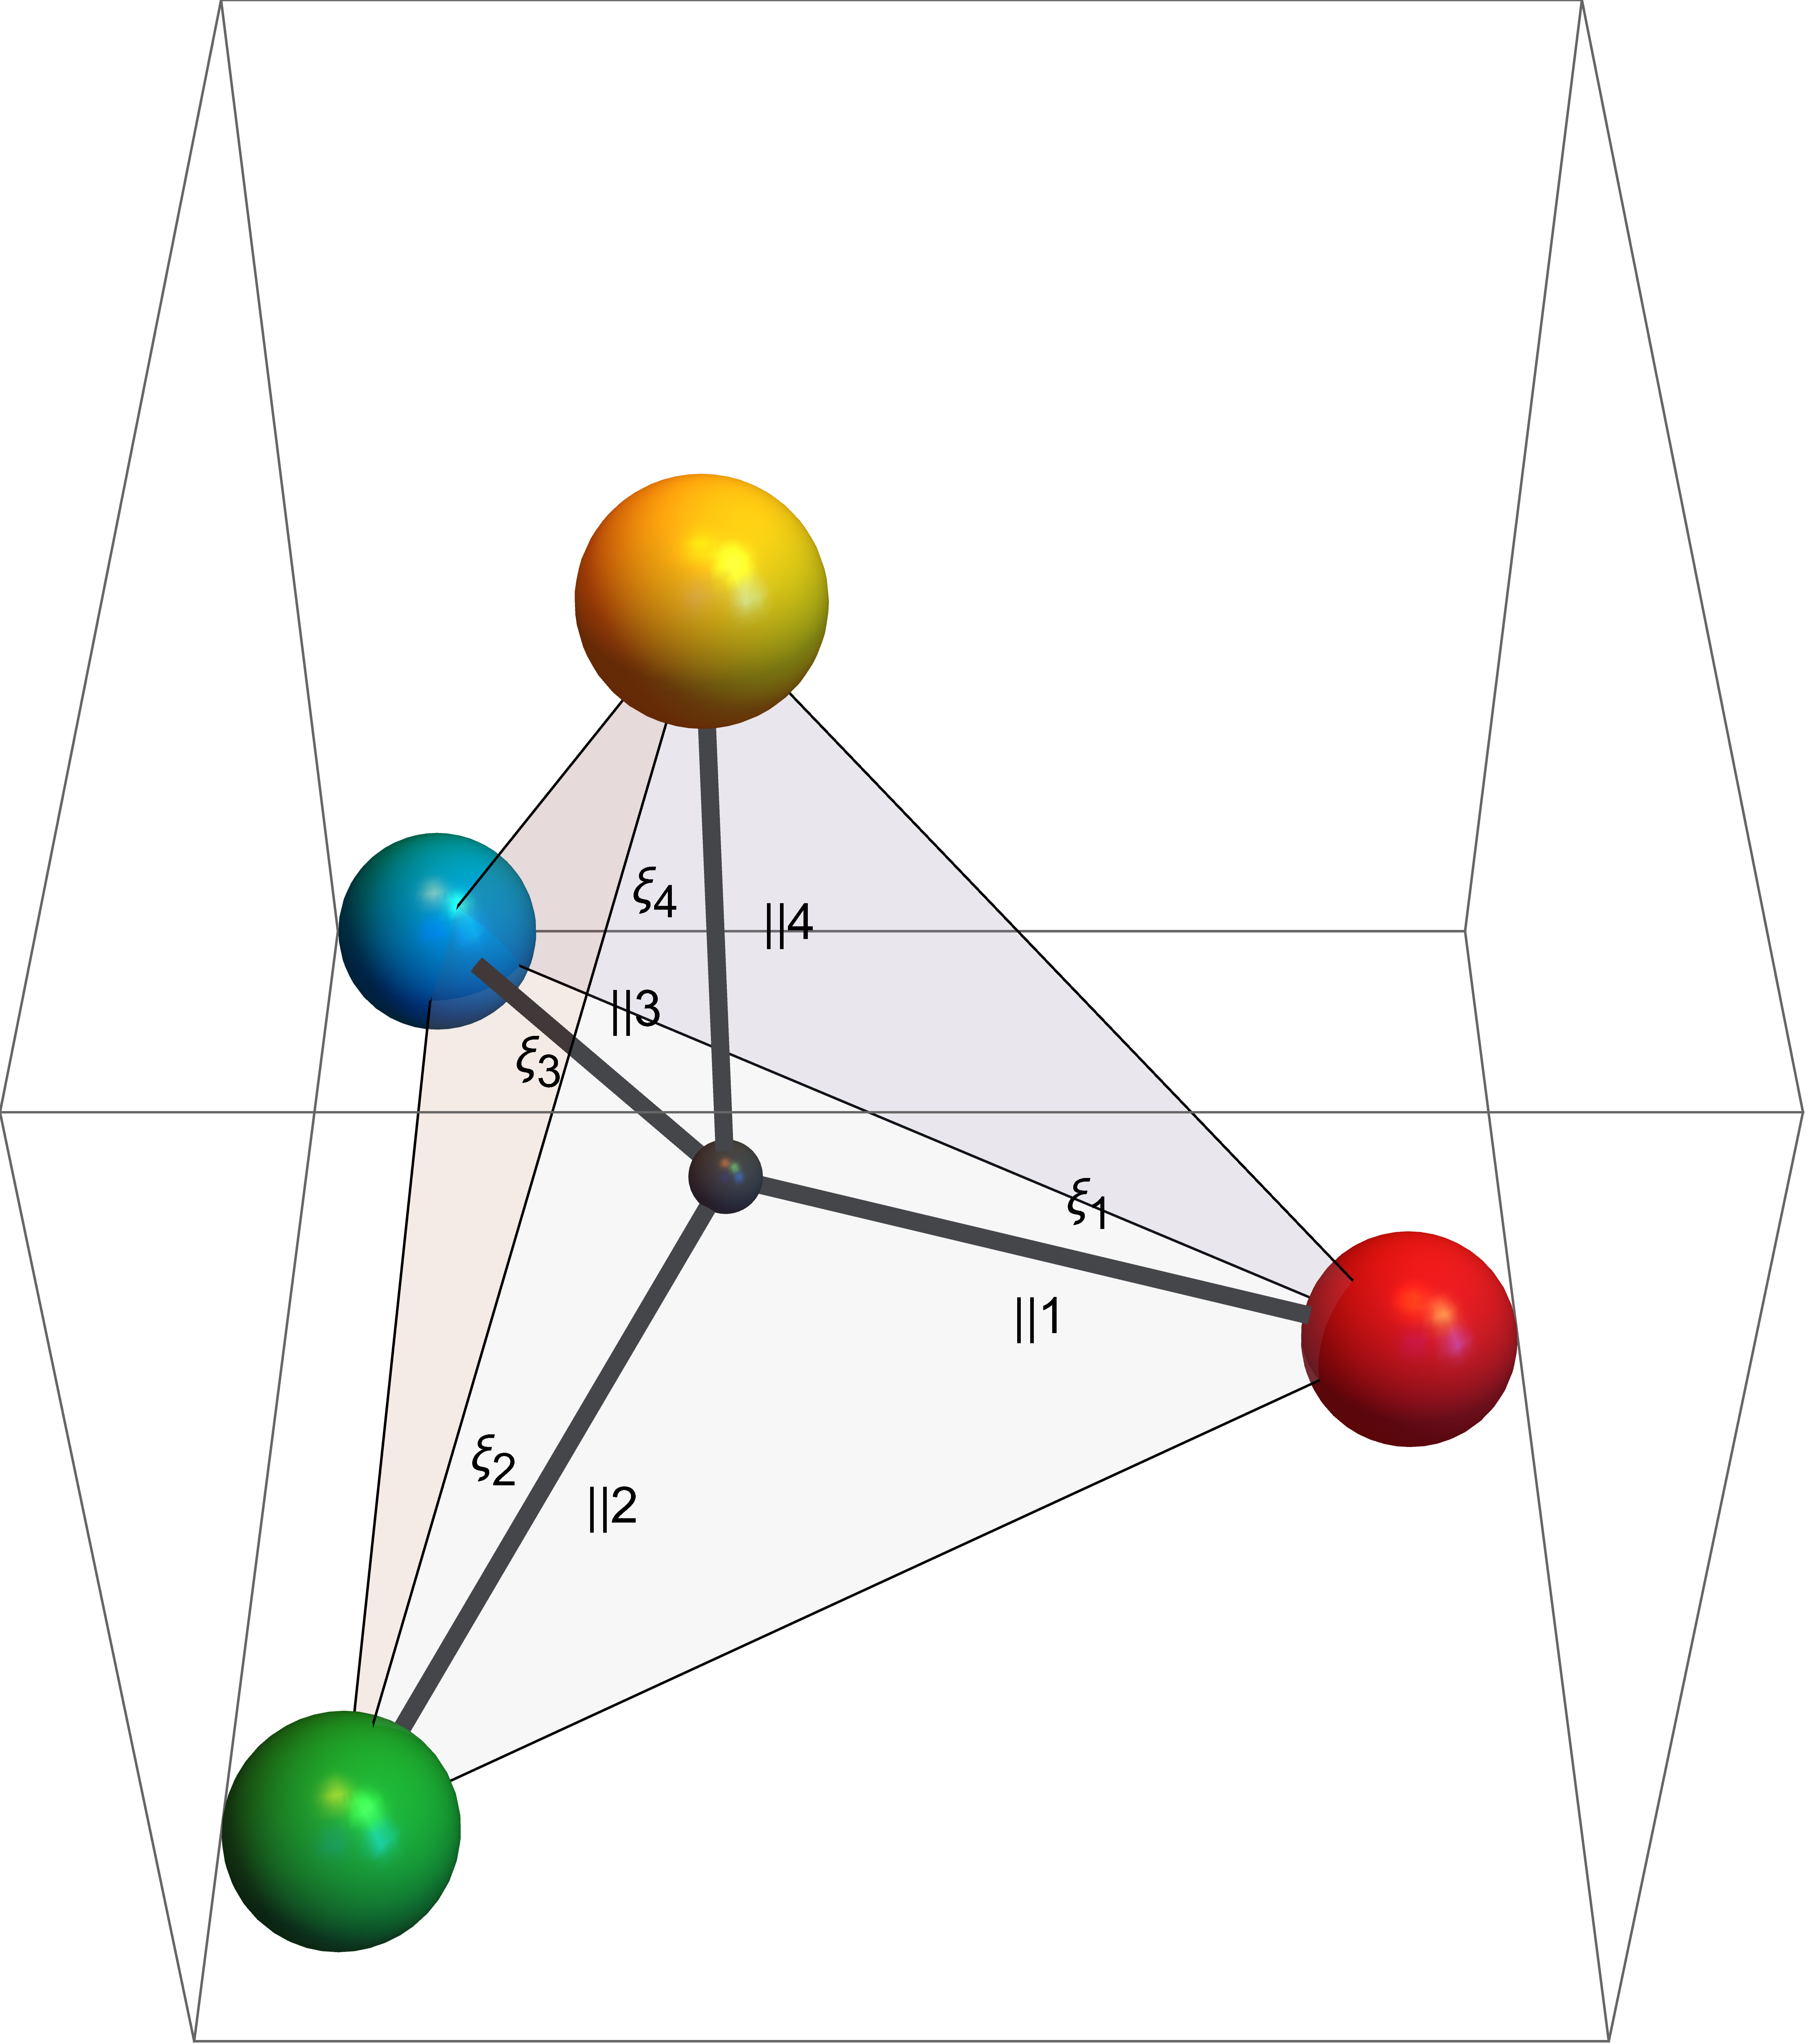
\includegraphics[height=1.5cm]{/Users/philipp/Documents/GitHub/stage_cmap/tex/Présentation/images/spr4nolabel.png}}

% bibliography
\usepackage[style = ieee, sorting = nty, backend = biber]{biblatex}
\bibliography{/Users/philipp/Documents/GitHub/stage_cmap/tex/Report/report.bib}
\usepackage{csquotes}

% environments

% proposition
\theoremstyle{plain}
\newtheorem{proposition}{Proposition}[section]

\setbeamertemplate{theorems}[numbered]


% additional packages
\usepackage{appendix}
\usepackage{amsmath}
\usepackage{amsfonts}
\usepackage{amssymb}
\usepackage{amsthm}
\usepackage{booktabs}
\usepackage{subfig}

\newcommand{\N}{\mathbb{N}}
\newcommand{\M}{\mathcal{M}}
\newcommand{\R}{\mathbb{R}}
\newcommand{\h}{\mathcal{H}}
\newcommand{\K}{\mathcal{K}}
\DeclareMathOperator{\Skew}{Skew}
\DeclareMathOperator{\id}{id}
\newcommand{\so}{\mathfrak{so}}
\newcommand{\REF}{\mathrm{ref}}
\newcommand{\spr}{\textsc{SPr4}}
\DeclareMathOperator{\dist}{dist}
\DeclareMathOperator{\SO}{SO}
\DeclareMathOperator{\sgn}{sgn}
\DeclareMathOperator{\Aut}{Aut}
\DeclareMathOperator{\diag}{diag}
\newcommand{\chroexp}{\overset{\longrightarrow}{\exp}}
\DeclareMathOperator{\re}{Re}
\DeclareMathOperator{\Span}{span}
\newcommand{\dd}[1]{\mathrm{d}#1}
\DeclareMathOperator{\ad}{ad}
\newcommand{\T}{\mathcal{T}}

\begin{document}

\maketitle


\section[Introduction]{Introduction}

\begin{frame}{Introduction}
\begin{itemize}
\item Premiers résultats sur le sujet par Purcell en 1977, en particulier le "scallop theorem"
\item Analyse (partielle) de plusieurs mécanismes de micro-natation
\end{itemize}
\begin{figure}[h]
\centering
\subfloat[3S]{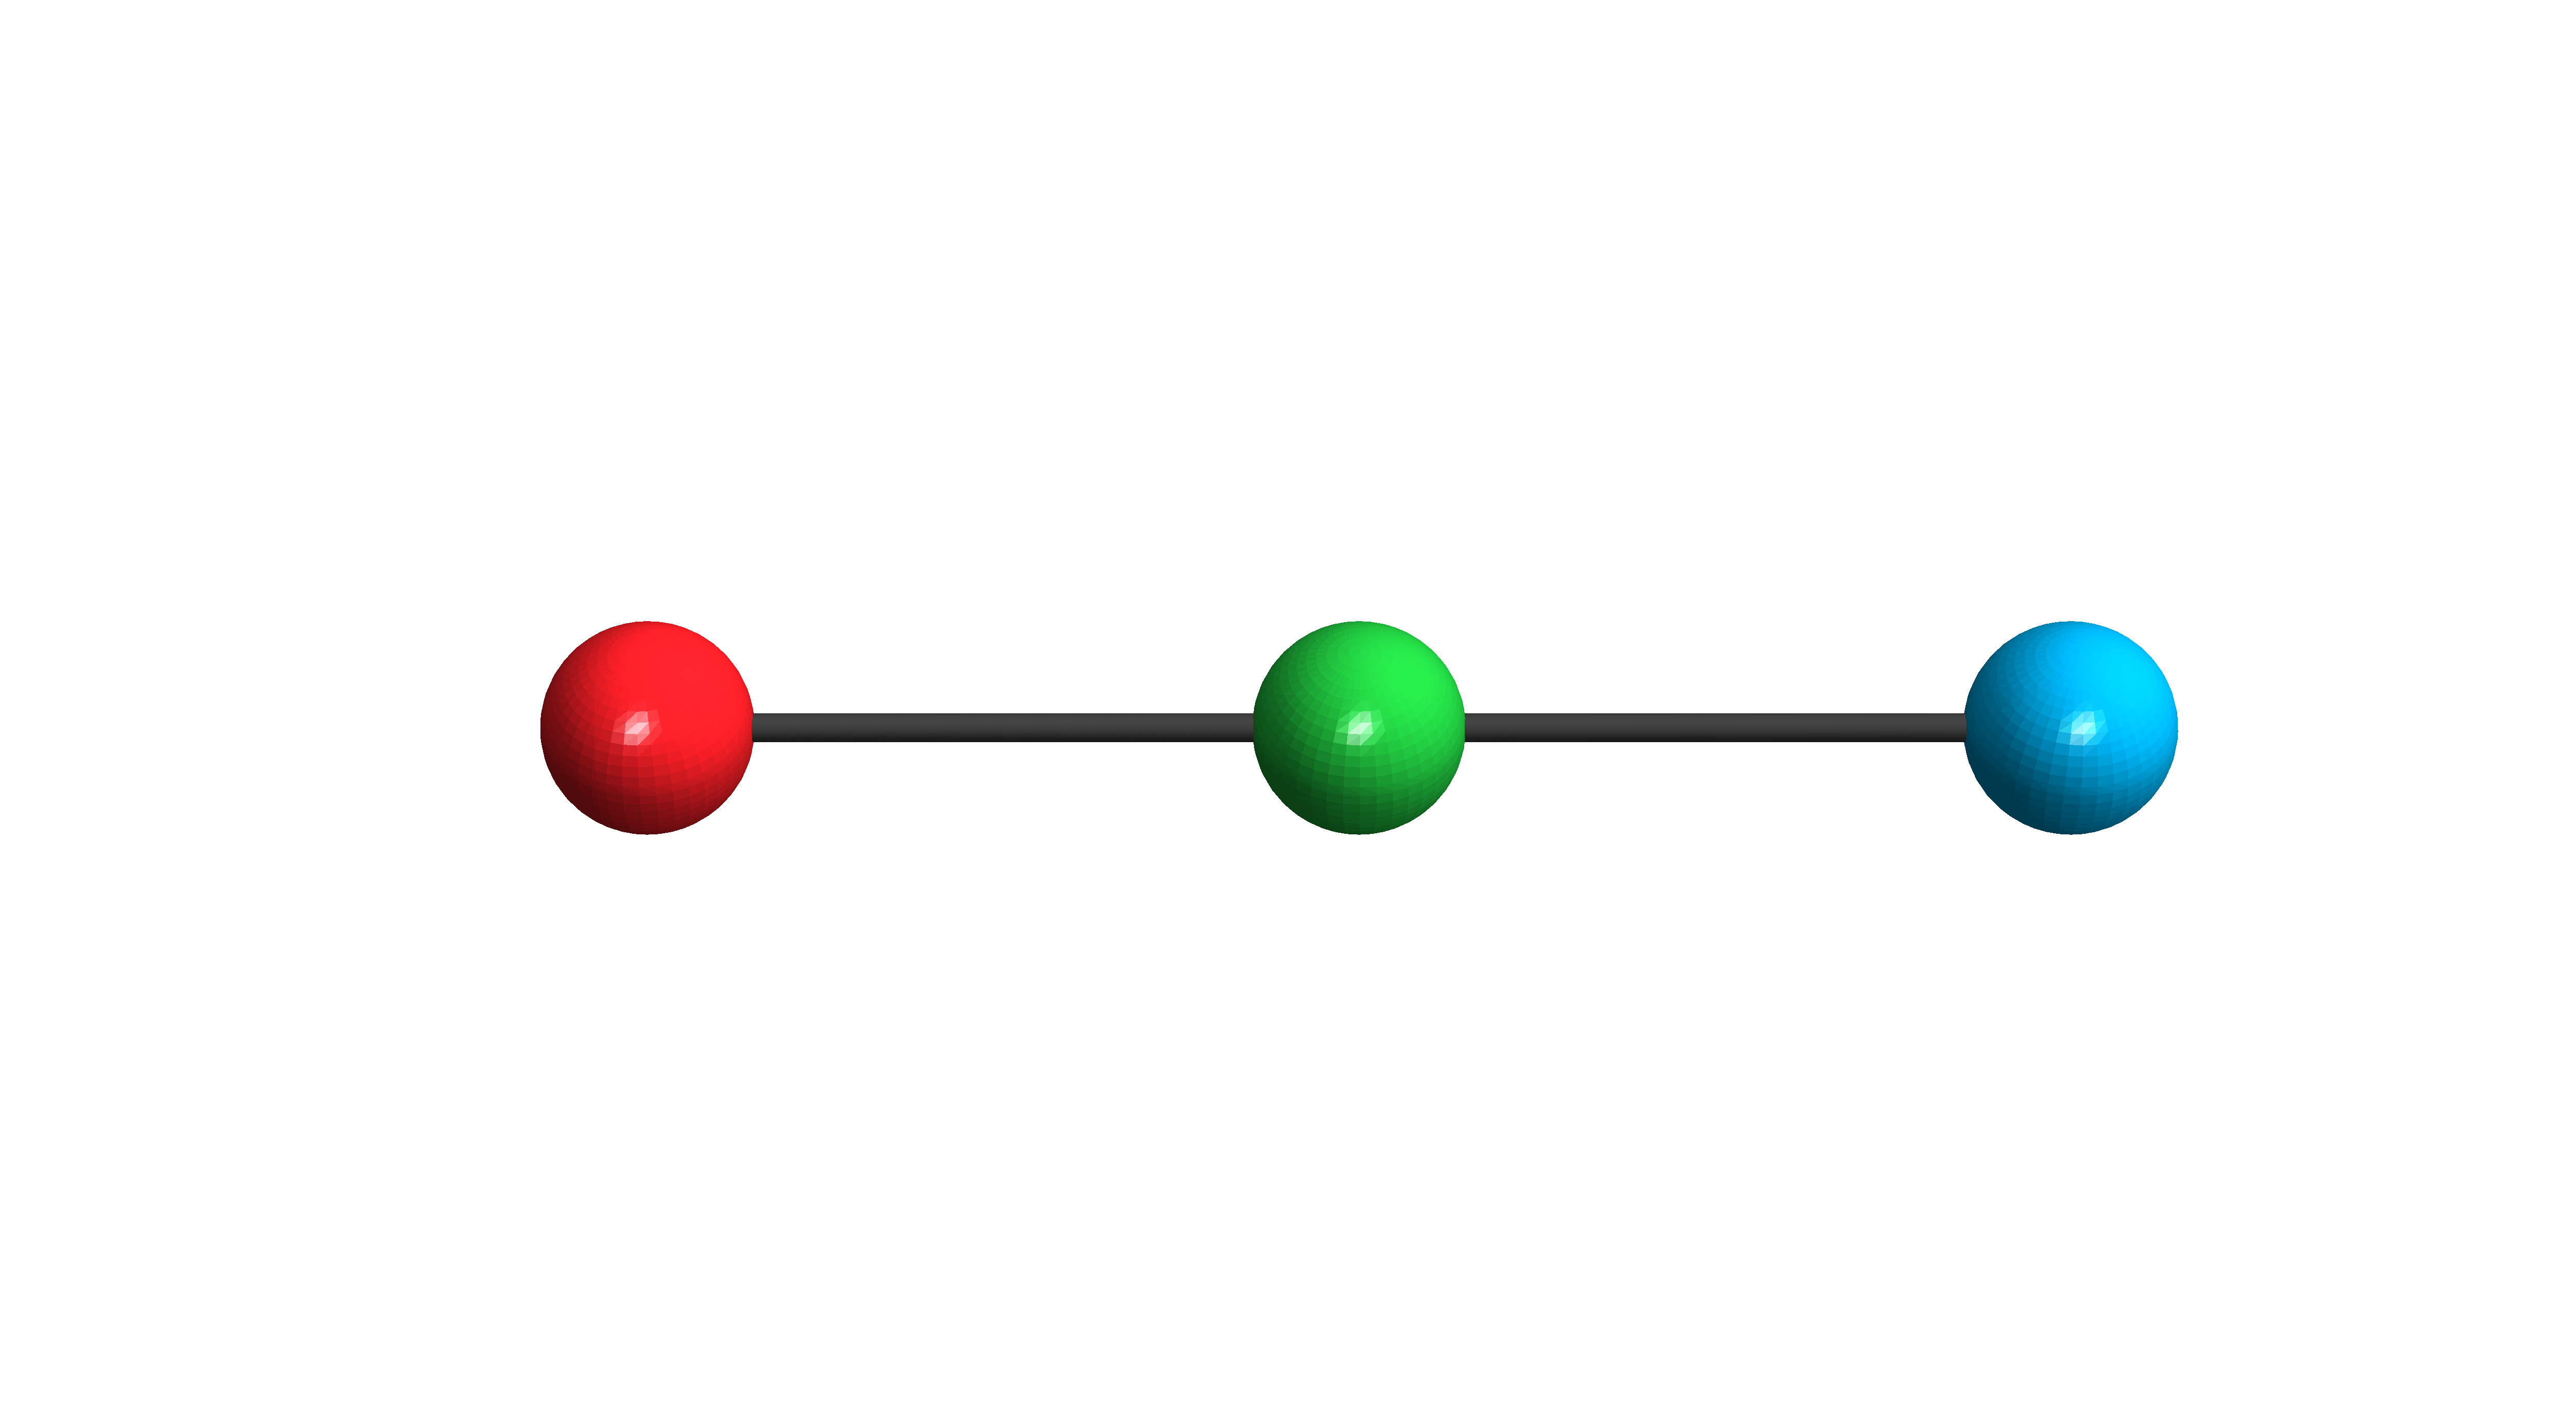
\includegraphics[width = 0.33\textwidth]{/Users/philipp/Documents/GitHub/stage_cmap/tex/Présentation/images/3s_nolabel.png}} 
\subfloat[SPr3]{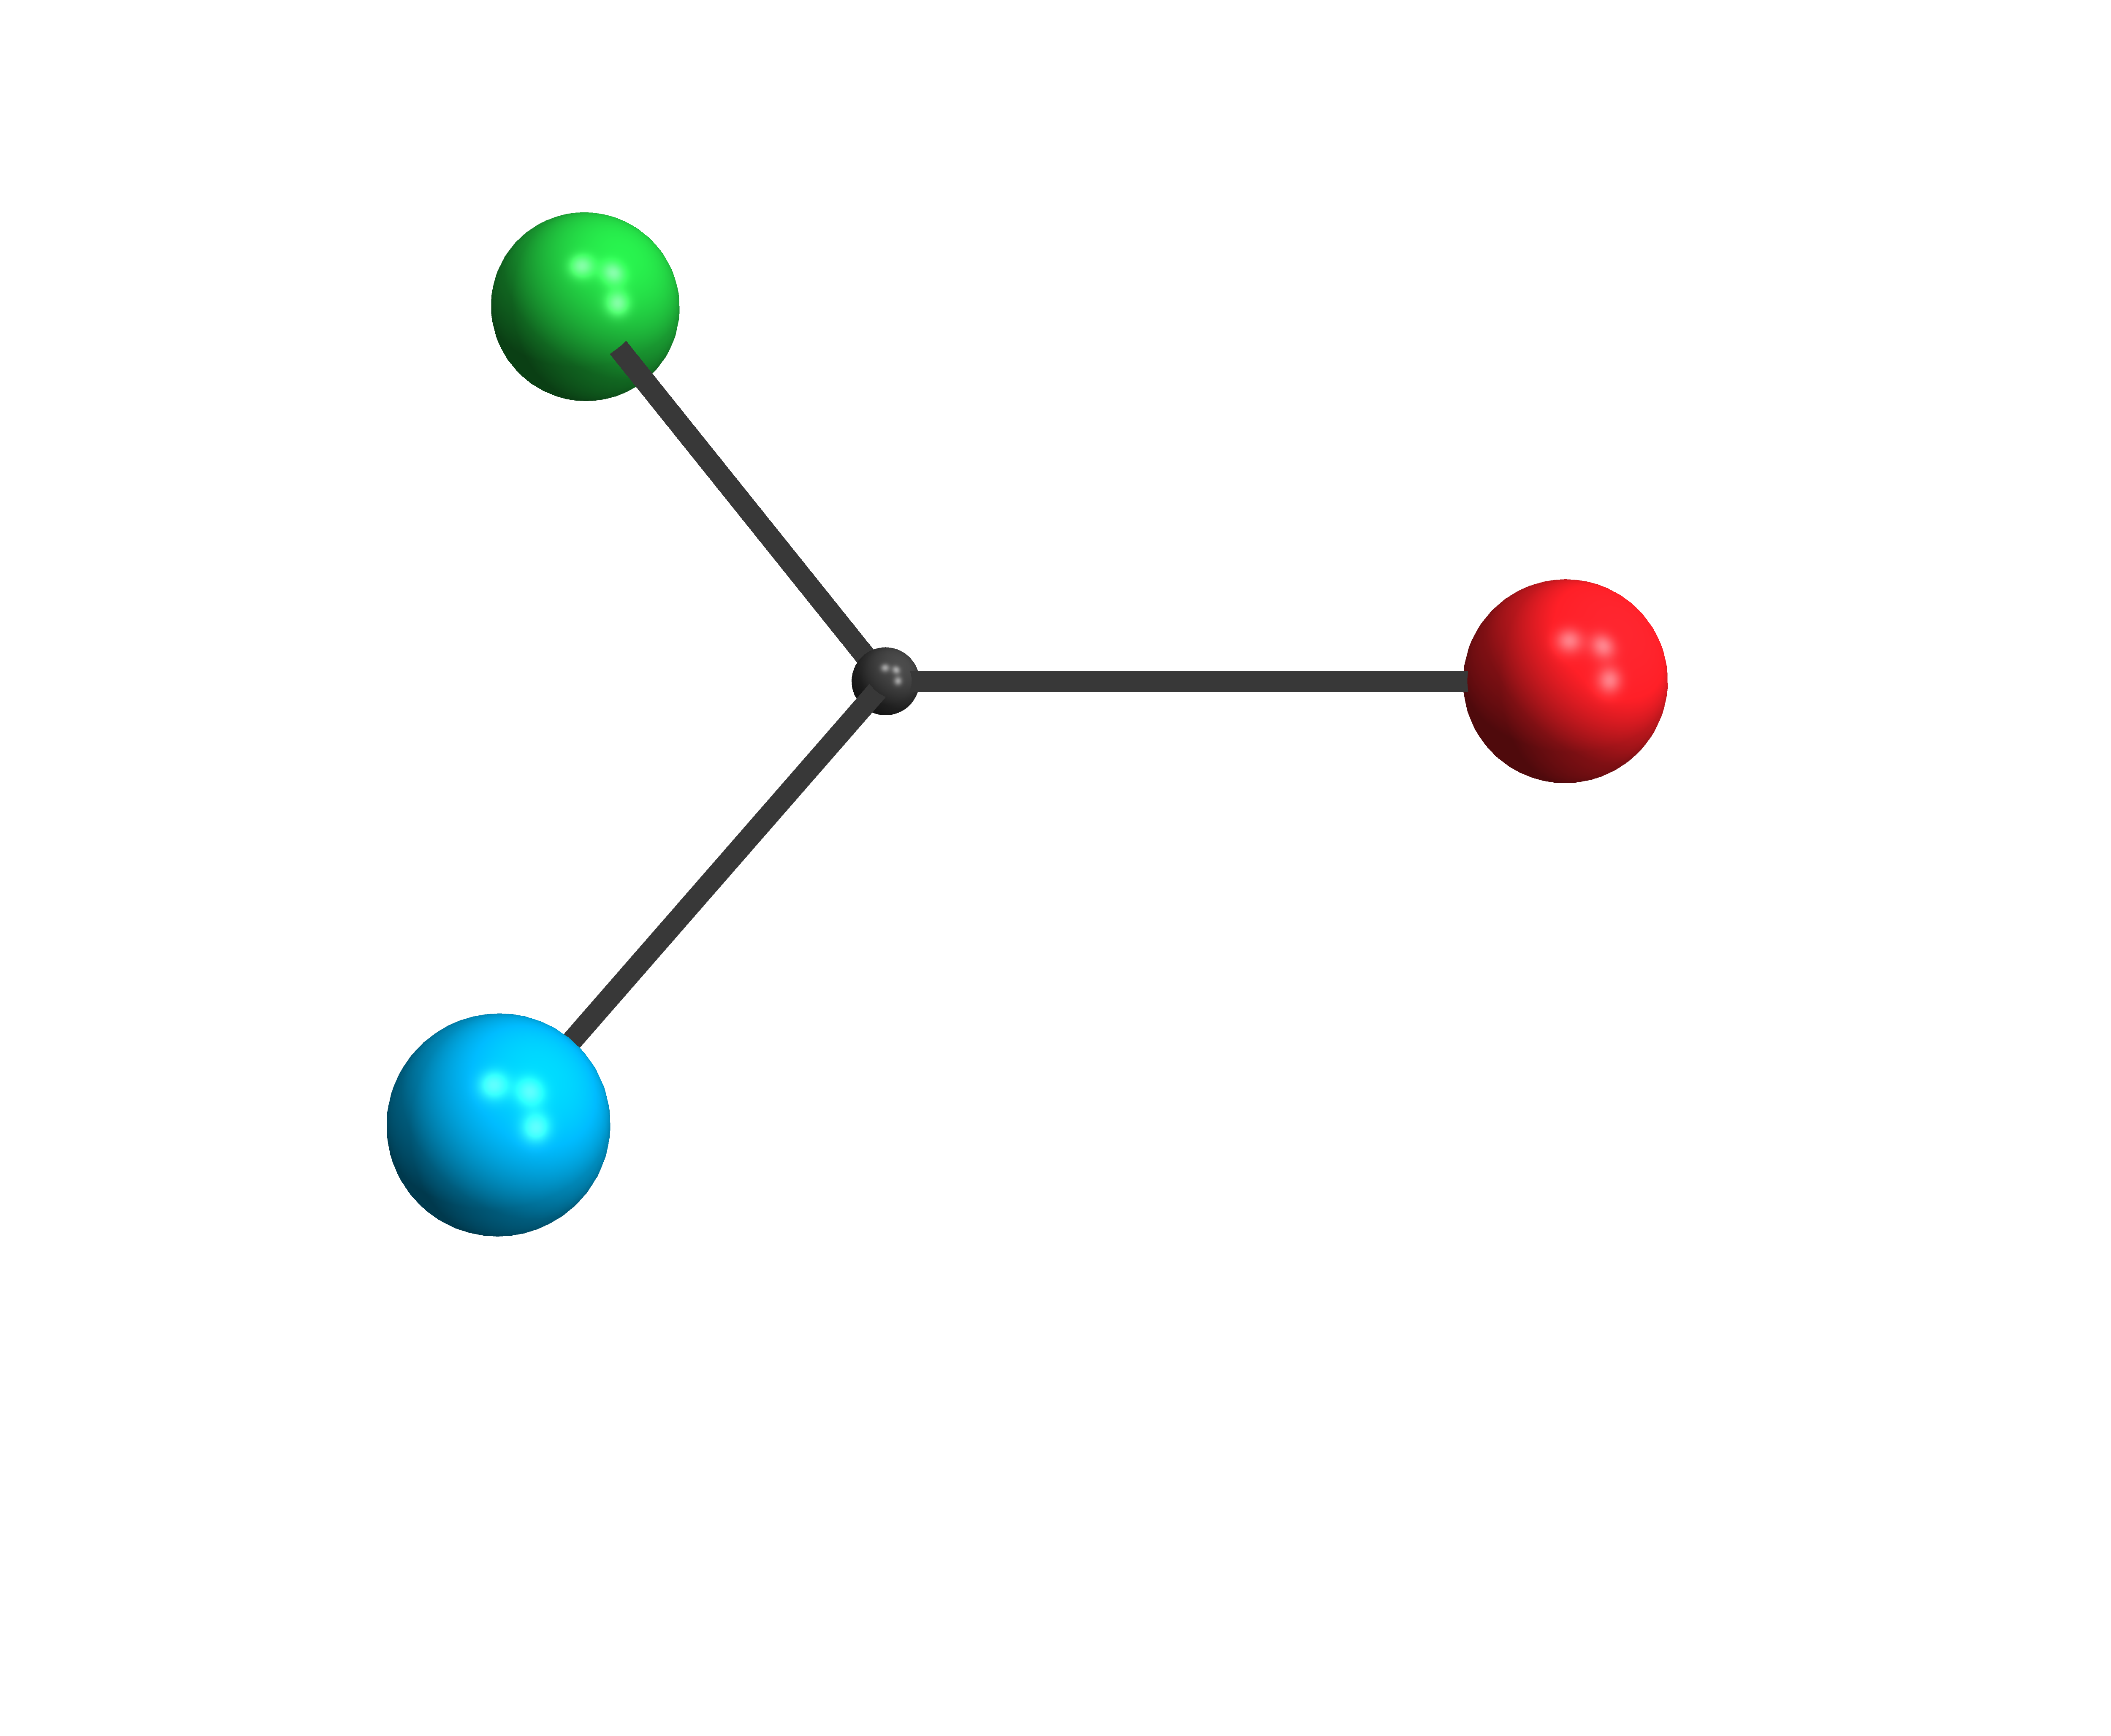
\includegraphics[width = 0.33\textwidth]{/Users/philipp/Documents/GitHub/stage_cmap/tex/Présentation/images/spr3nolabel.png}}
\subfloat[SPr4]{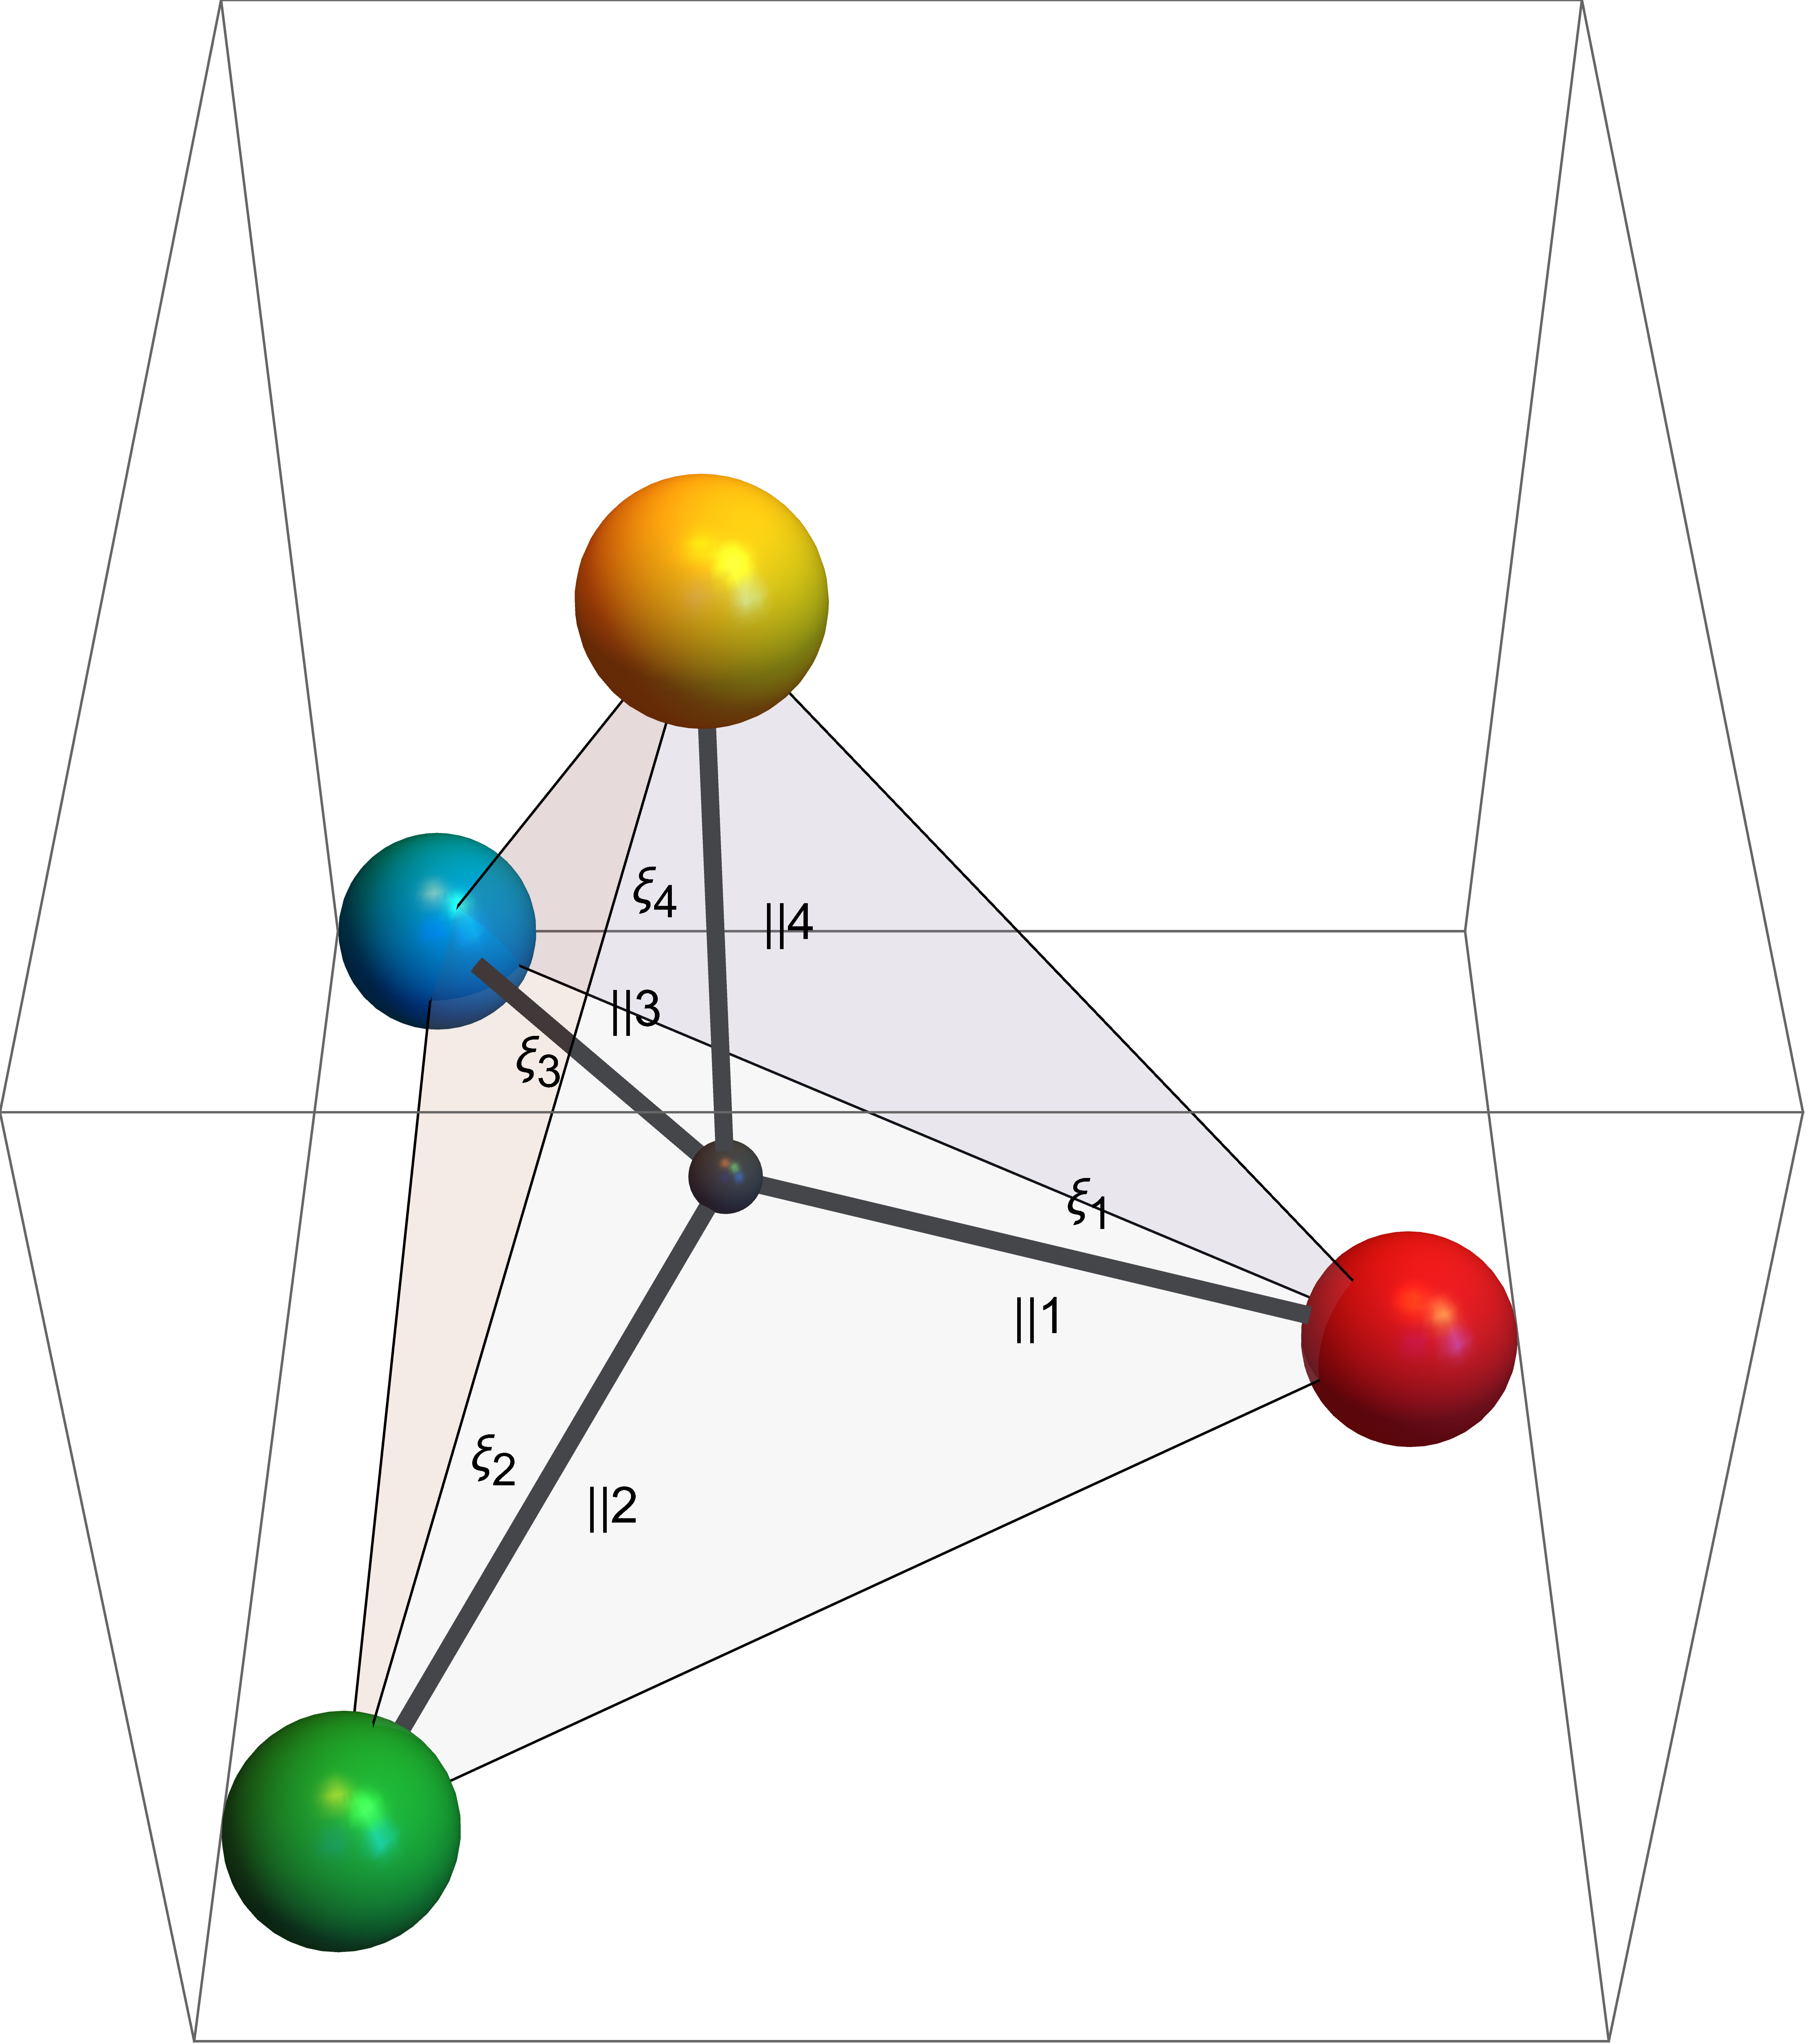
\includegraphics[width = 0.33\textwidth]{/Users/philipp/Documents/GitHub/stage_cmap/tex/Présentation/images/spr4nolabel.png}}
\caption{Exemples de micro-nageurs}
\label{fig:swimmers}
\end{figure}


\end{frame}

\begin{frame}{Introduction}
\begin{itemize}
\item Problème mathématique: $\re \ll 1 \implies$ forces d'inertie négligeables
\item Problème de contrôle
\item Question supplémentaire: Natation optimal, i.e. problème de contrôle optimale
\item Contrôlabilité globale de \textsc{SPr4} démontré dans \cite{Alouges2013}, mais pas explicitement
\item Dans ce projet: Analyse du nageur \textsc{SPr4} sous l'hypothèse des mouvements petits de la structure des courbes de contrôle optimales pour une classe particulière de déplacements prescrits.
\end{itemize}
\end{frame}

\begin{frame}{Table des matières}
  \setbeamertemplate{section in toc}[sections numbered]
  \tableofcontents[hideallsubsections]
\end{frame}


\section{Modélisation et symétries}

\begin{frame}{Notation et modèle}
\begin{itemize}
\item Tétraèdre de référence avec sommets $(S_1, S_2, S_3, S_4)$ centré à $c \in \R^3$ tel que $\dist(c, S_i) = 1$
\item Quatre boules $B_i$, centrées à $b_i$ de rayon $a > 0$ peuvent bouger le long de la demi-droite d'origine $c$ passant par $S_i$
\item La résistance visqueuse des bras est négligée
\item Description complète par deux ensembles de variables:
\begin{enumerate}
\item \emph{Les variables de forme:} $\xi := (\xi_1, \xi_2, \xi_3, \xi_4) \in \M := (\sqrt{3/2}a, + \infty)^4$, où les $\xi_i$ sont les longueurs des bras.

\item \emph{Les variables de position:} $p = (c, R) \in \mathcal{P} := \R^3 \times \SO(3)$.
\end{enumerate}
\item $z_i := \overline{c S_i}$
\end{itemize}

\end{frame}

\begin{frame}{Notation et modèle}
\begin{figure}[h]
    \centering
    \begin{minipage}{0.45\textwidth}
        \centering
        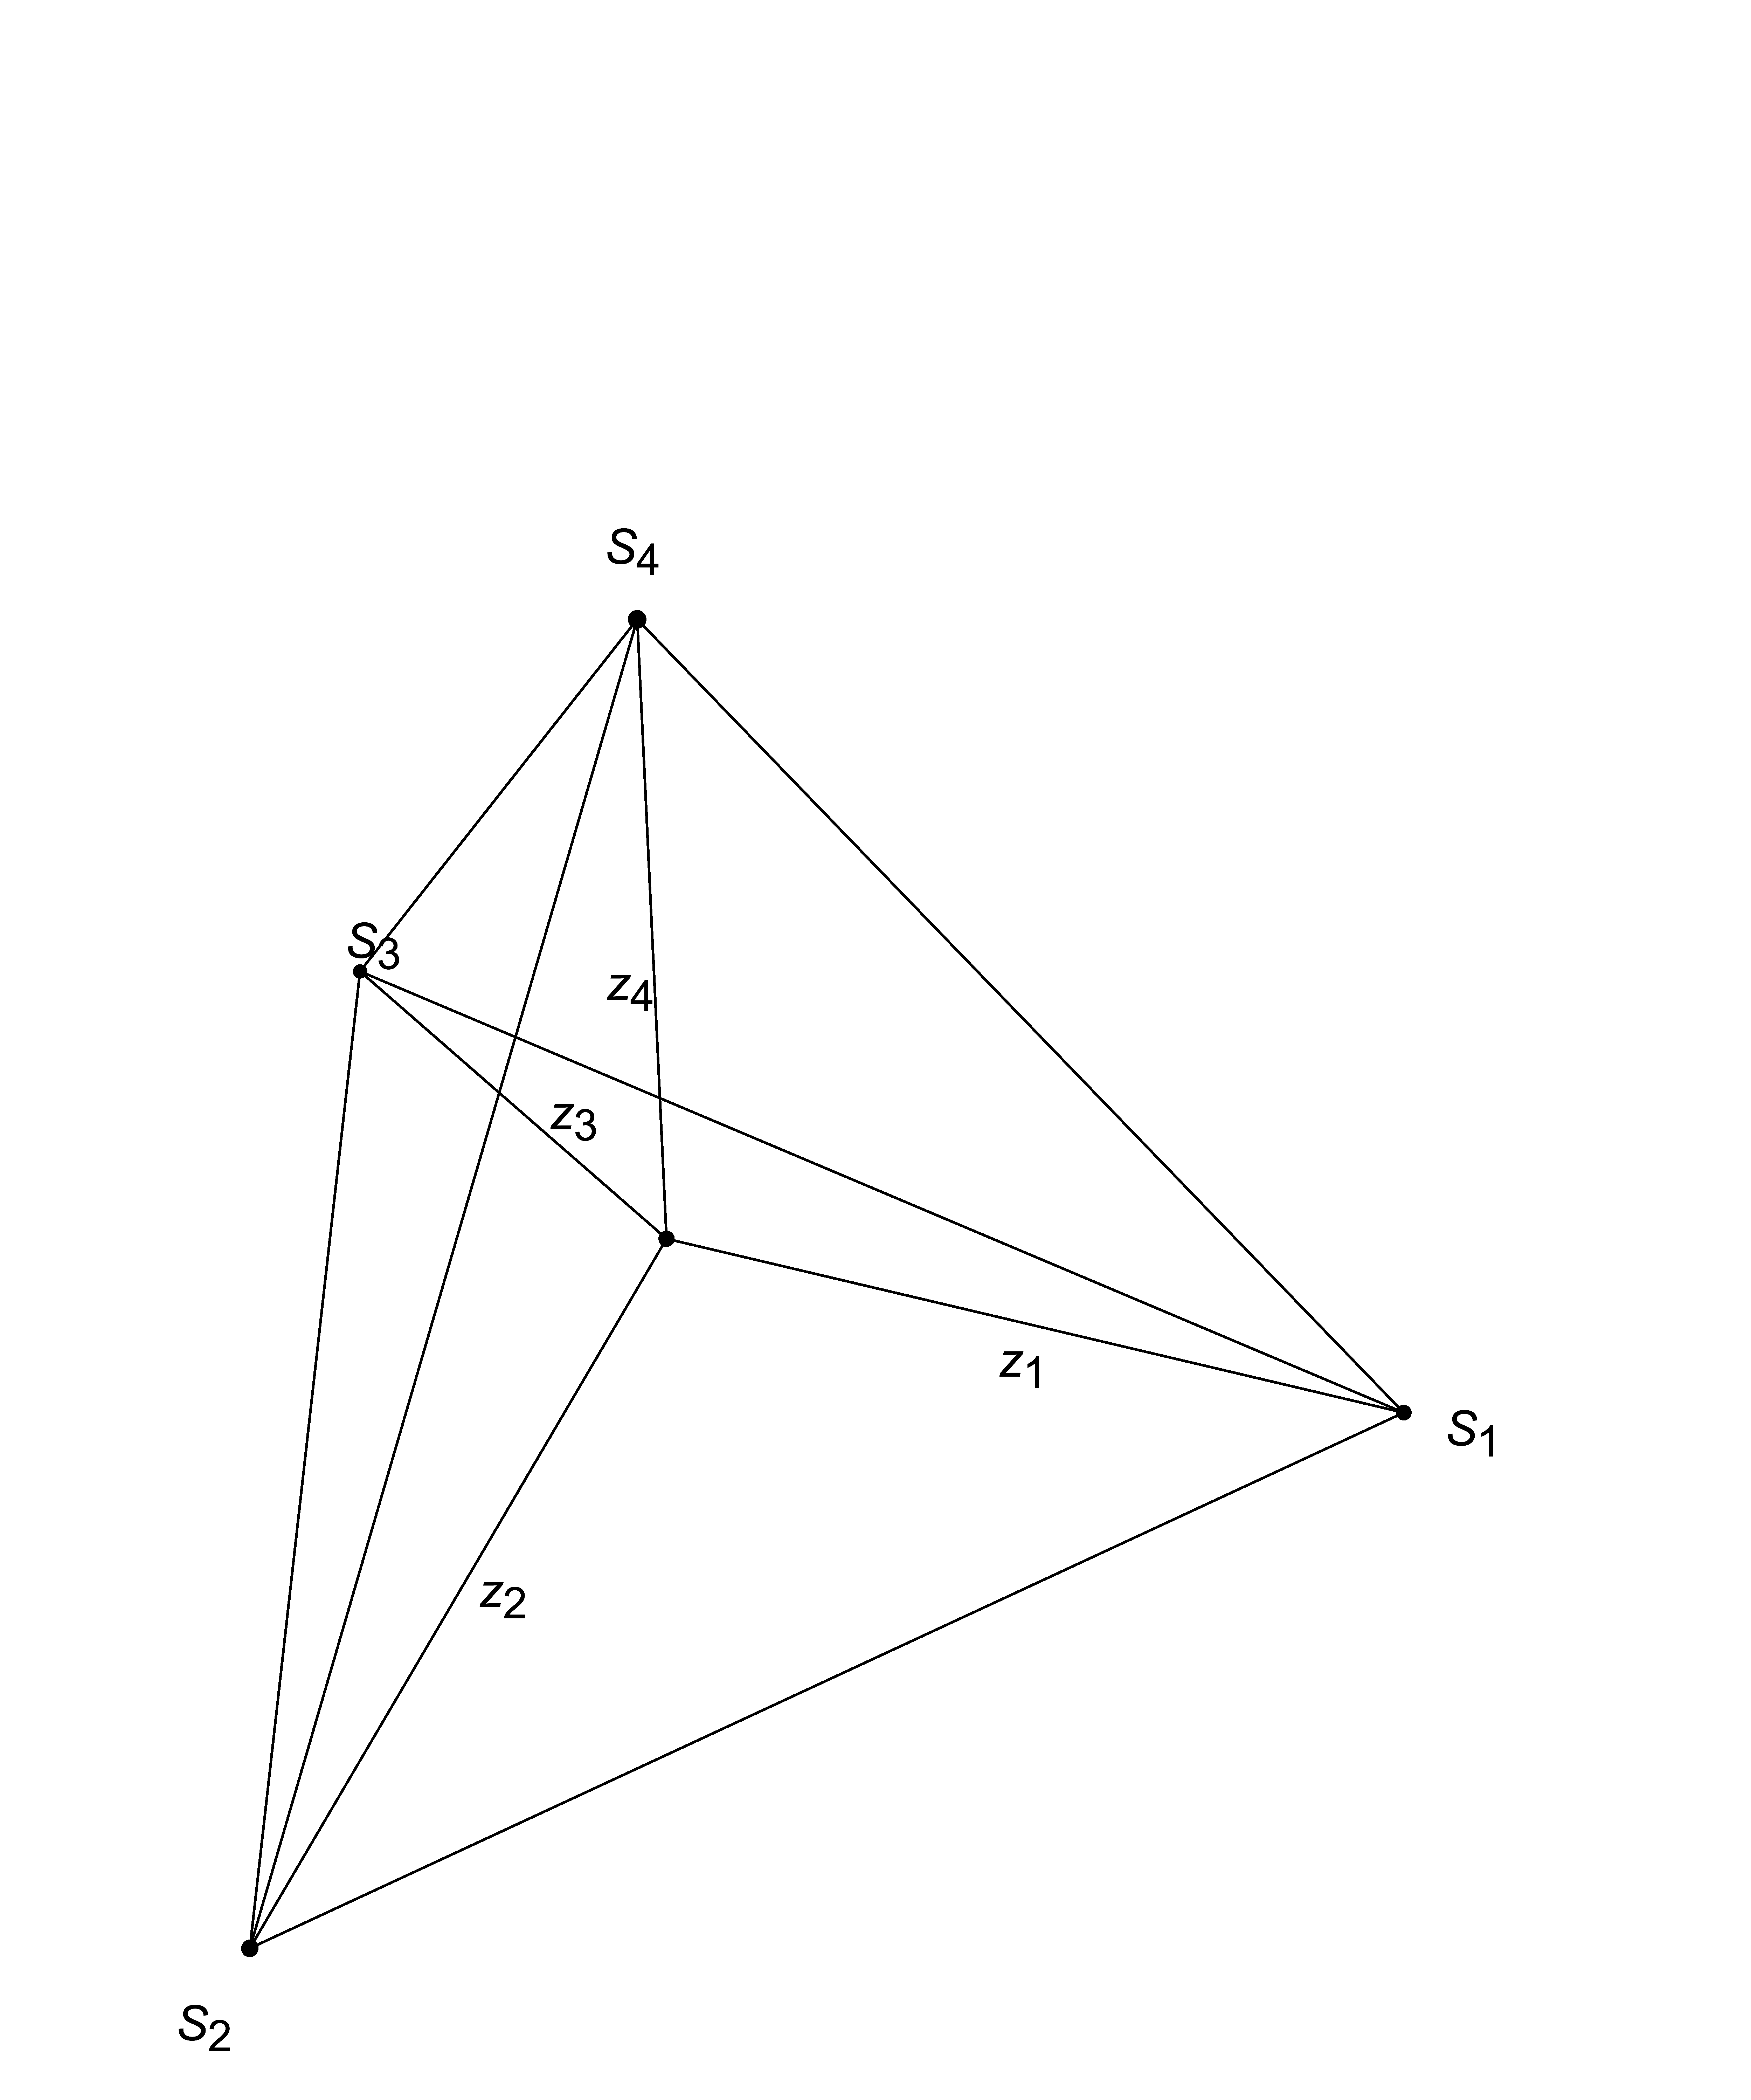
\includegraphics[width=0.9\textwidth]{/Users/philipp/Documents/GitHub/stage_cmap/images/tetrahedron.png}
    \end{minipage}
    \begin{minipage}{0.45\textwidth}
        \centering
        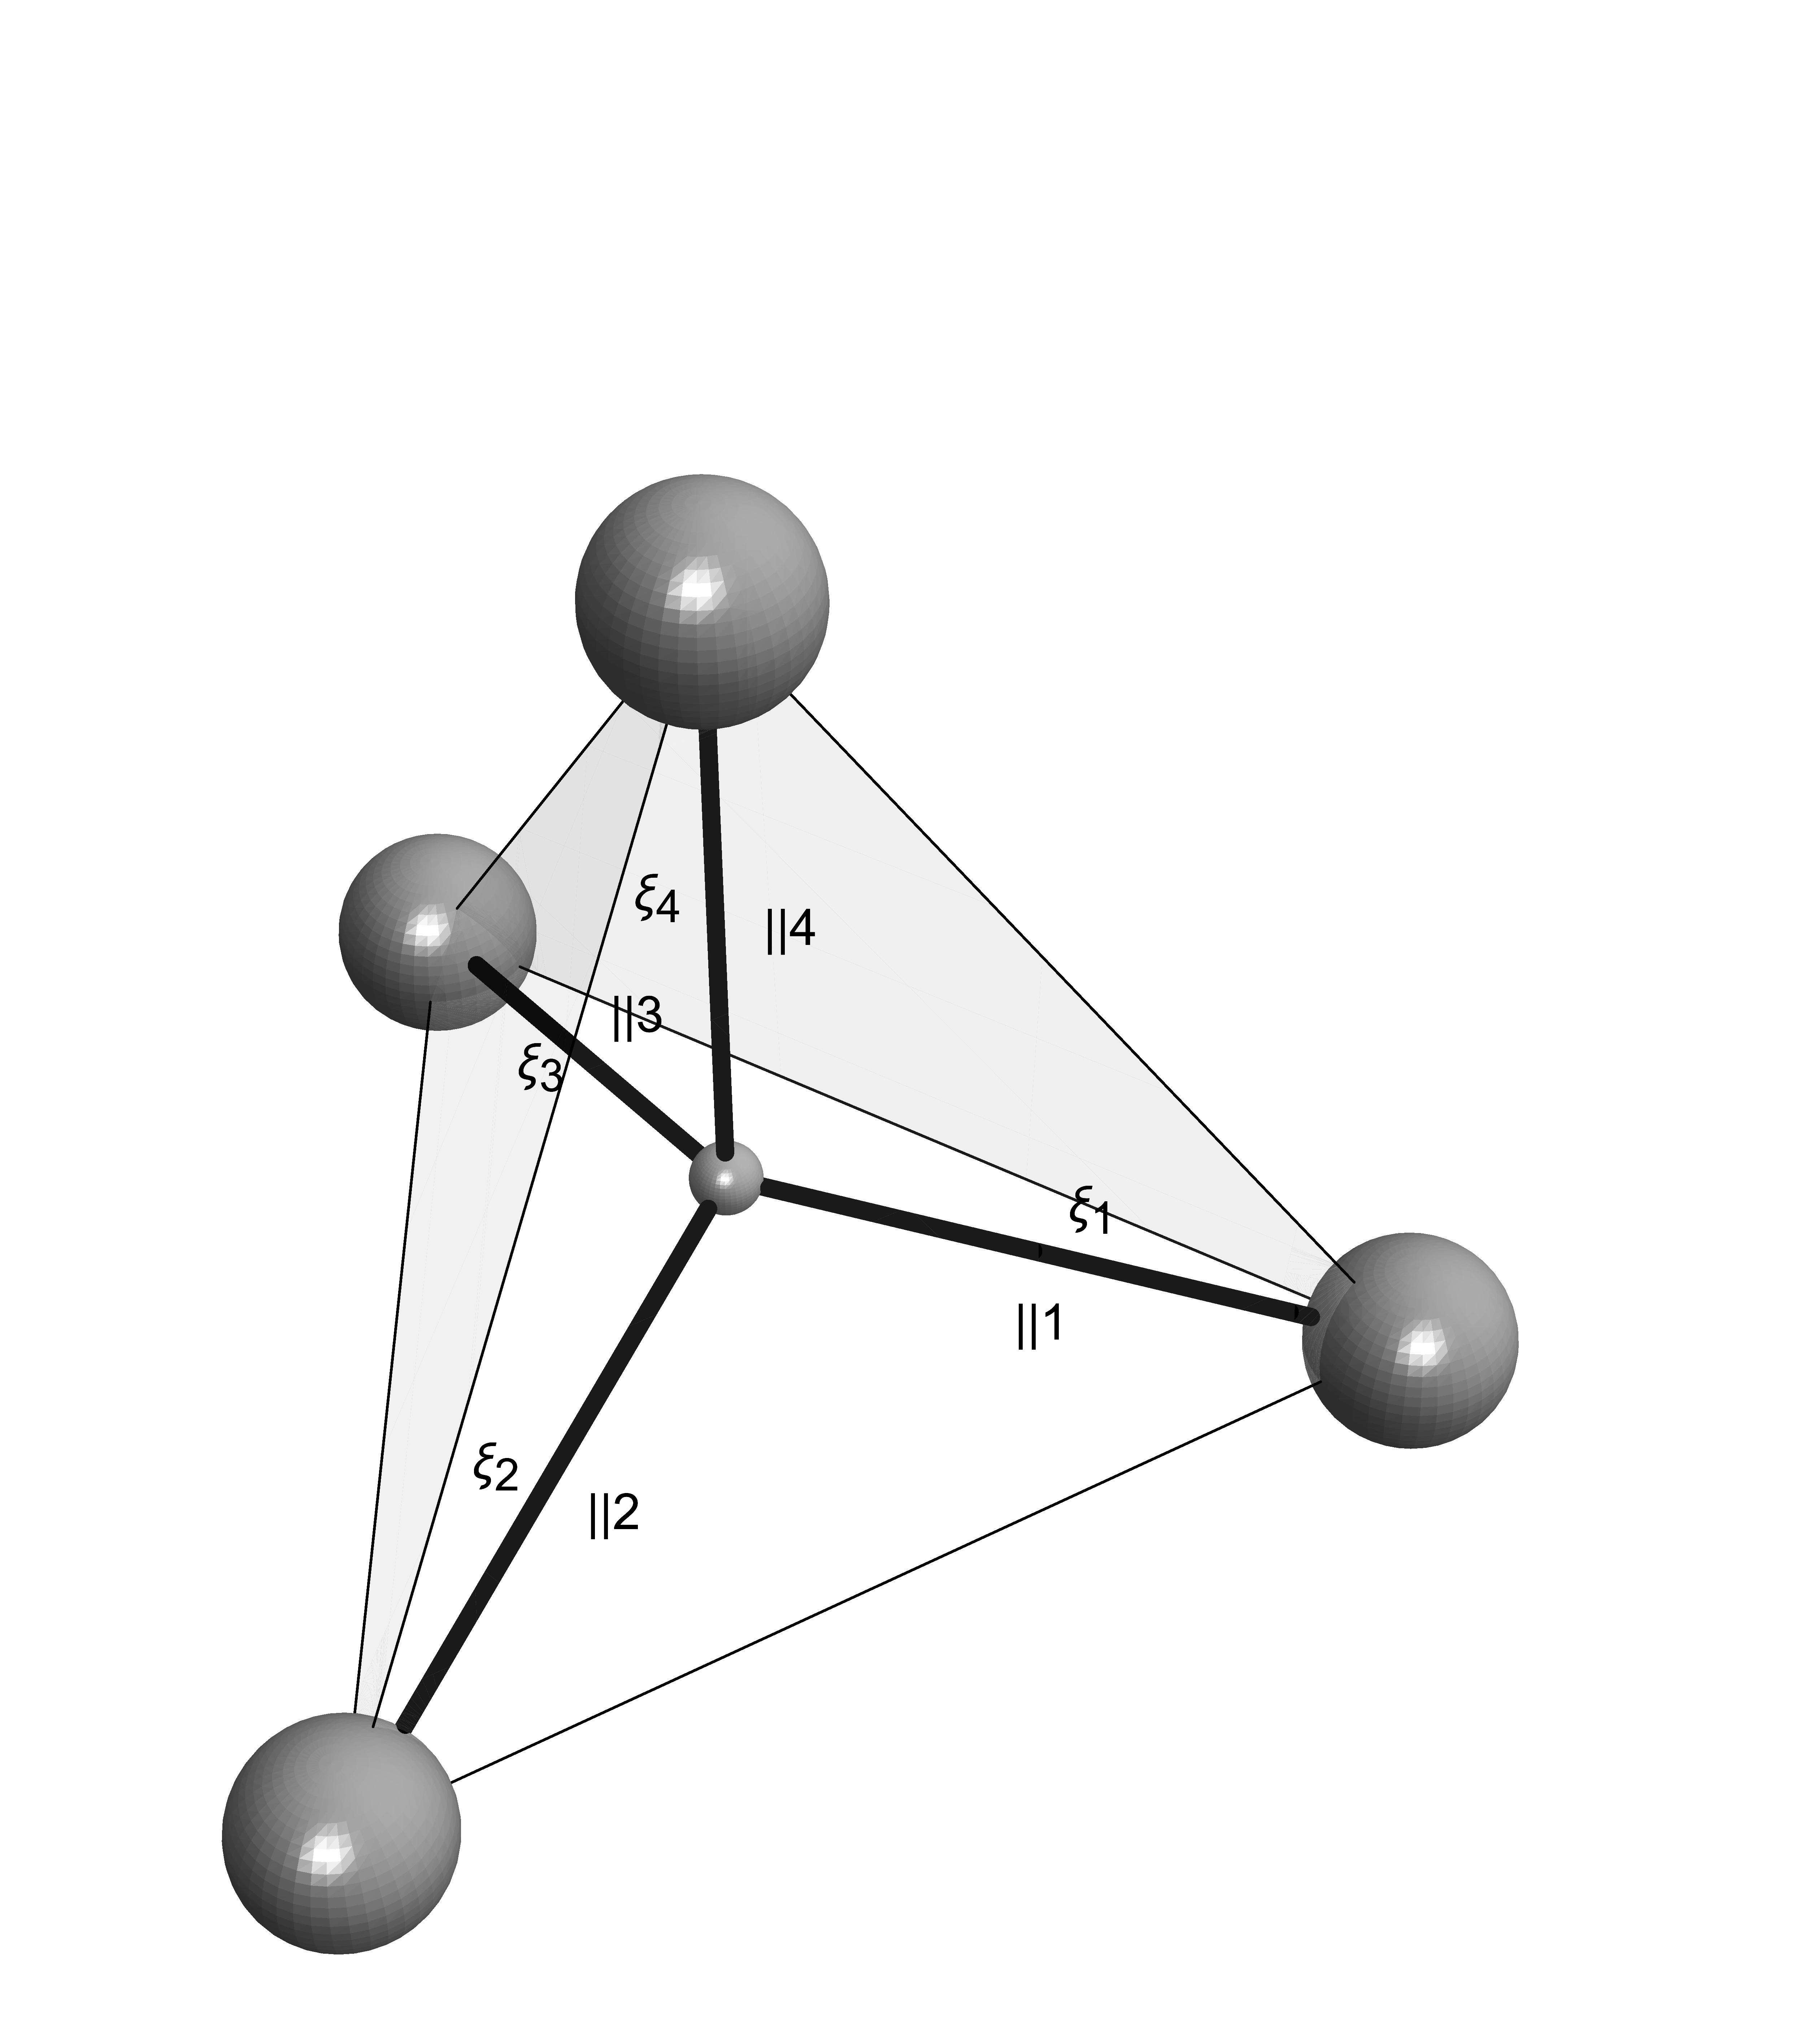
\includegraphics[width=0.9\textwidth]{/Users/philipp/Documents/GitHub/stage_cmap/images/spr4.png} % second figure itself
    \end{minipage}
    \caption{Le tétraèdre de référence et le "parking 4-sphere swimmer" (\textsc{SPr4}).}
    \label{fig:reference tetrahedron and spr4}
\end{figure}

\end{frame}

%\begin{frame}{Notation et modèle}
%\begin{itemize}
%\item Soit $r \in B_a$, la boule centrée à l'origine de rayon $a > 0$. Le point actuel sur $B_i$ est donné par
%\begin{equation}
%	r_i(\xi, p, r) :=  c + R(\xi_i z_i + r).
%\end{equation}
%\item Les $r_i$ sont analytiques $\to$ déduire la vitesse instantanée
%\begin{equation}
%	u_i(\xi, p, r) = \dot{c} + \omega \times (\xi_i z_i + r) + R z_i \dot{\xi}_i,
%\end{equation}
%où $\omega$ est le vecteur axial associé à la matrice anti-symétrique $\dot{R}R$.
%\end{itemize}
%
%\end{frame}

\begin{frame}{Notation et modèle}
\begin{itemize}
\item Système dynamique trouvé dans \cite{Alouges2013}
\begin{equation}
\label{eq: control system}
	\dot{p} = F(R, \xi) \dot{\xi} := \left ( \begin{array}{c}
	F_c(R, \xi) \\
	F_\theta(R, \xi)
	\end{array}  \right ) \dot{\xi},
\end{equation}
tel que $\dot{c} = F_{c}(R, \xi) \dot{\xi}$ et $\dot{R} =F_{\theta}(R, \xi) \dot{\xi}$.
\item \begin{equation}
\begin{aligned}
	F_c(R, \xi) \in \mathcal{L}(\R^4, \R^3) \text{ et } F_{\theta}(R, \xi) \in \mathcal{L}(\R^4,T_R \SO(3)).
\end{aligned}
\end{equation}
Donc, dès qu'on a fixé des bases, on peut les exprimer comme des matrices de taille $3 \times 4$.

%\item Pour $R \in \SO(3)$ fixé, on a
%\begin{align}
%T_{R}SO(3) = \{R M \mid M \in \Skew_3(\R)\}.
%\end{align}
%\item $\dim T_{R}\SO(3) = 3 \implies$ on peut exprimer $F_{c}(R, \xi), F_{\theta}(R,\xi)$ des matrices de taille $3 \times 4$, dès qu'on a choisi des bases
\end{itemize}

\end{frame}


\begin{frame}{Symétries}
%\begin{itemize}
%\item Condition initiale $p_0 = (c_0, R_0) \in \mathcal{P}$
%\item Courbe de contrôle $\xi: J \subset \R \to \M$, avec $J$ un voisinage de zéro
%
%\item $\gamma(c_0, R_0, \xi): I \to \mathcal{P}$ solution associée au système dynamique
%\begin{equation}
%\label{eq:dynamical system}
%\begin{aligned}
%	&\dot{p} = F(R, \xi) \dot{\xi},& & p(0) := p_0.
%\end{aligned}
%\end{equation}
%
%\item $\gamma_c(c_0, R_0, \xi)$ et $\gamma_{\theta}(c_0, R_0, \xi)$ les projections à $\R^3$ et $\SO(3)$
%
%\item Par définition, on a
%\begin{equation}
%	\dot{\gamma}(c_0, R_0, \xi)(t) = F(\gamma_\theta(c_0, R_0, \xi)(t), \xi(t))\dot{\xi}(t), \forall t \in J.
%\end{equation}
%\end{itemize}

\begin{itemize}
\item Investigation du système de contrôle (\ref{eq: control system}) sur la base des symétries des équations de Stokes
\item Équations de Stokes $\to$ invariantes sous rotations et changement de point de vue
\item Pour trouver les symétries de $F$ $\to$ appliquer les transformations correspondantes à une solution, puis différentiation
\end{itemize}
\end{frame}

\begin{frame}{Symétries - Invariance rotationnelle}
%\begin{itemize}
%\item Invariance rotationnelle des équations de Stokes $\implies$
%\begin{equation}
%\label{eq:spatial rotational invariance}
%	\gamma_c(c_0, R R_0, \xi)(t) = R \gamma_c (c_0, R_0, \xi)(t) + (I - R) c_0, \forall t \in J
%\end{equation}
%et
%\begin{equation}
%\label{eq: angular rotational invariance}
%	\gamma_\theta(c_0, R R_0, \xi)(t) =  R \gamma_\theta(c_0, R_0, \xi)(t), \forall t \in J
%\end{equation}
%\item Un calcul montre
%\begin{eqnarray}
%	F_c(R, \xi) = R F_c(\xi) \text { and } F_\theta(R, \xi) = R F_{\theta} (R, \xi),&  \forall (R, \xi) \in \SO(3) \times \M,
%\end{eqnarray}
%où $F_c(\xi) := F_{c}(I, \xi)$ et $F_{\theta}(\xi) := F_{\theta}(I, \xi)$.
%\end{itemize}

Pour toute rotation $R \in \SO(3)$, on trouve
\begin{eqnarray}
	F_c(R, \xi) = R F_c(\xi) \text { and } F_\theta(R, \xi) = R F_{\theta} (R, \xi),&  \forall (R, \xi) \in \SO(3) \times \M,
\end{eqnarray}
où $F_c(\xi) := F_{c}(I, \xi)$ et $F_{\theta}(\xi) := F_{\theta}(I, \xi)$.

\end{frame}


\begin{frame}{Symétries - Permutation des bras $||i \leftrightsquigarrow ||j$}
\begin{itemize}
\item Utiliser l'invariance sous changement de point de vue pour déterminer la symétrie de $F$ sous permutation de deux bras
\item $P_{ij} \in M_{4 \times 4}(\R)$ matrice de permutation t.q. les indices $i$ et $j$ sont échangés
\item $S_{ij}$ la réflexion t.q. $||i \mapsto ||j$ et vice-versa dans l'orientation de référence $I$.

%\item Les équations de Stokes sont invariantes sous changement de point de vue. Avec la position initiale $p_0 := (c, I)$ on en déduit que
%\begin{equation}
%\label{eq:spatial_perm_inv}
%	\gamma_c(c_0, I, P_{ij} \xi) = S_{ij} \gamma_c(S_{ij}c_0, I, \xi)
%\end{equation}
%et
%\begin{equation}
%\label{eq:angular_perm_inv}
%	\gamma_{\theta}(c_0, I, P_{ij} \xi ) = S_{ij} \gamma_{\theta} (S_{ij} c_0, I, \xi) S_{ij}.
%\end{equation}

\end{itemize}
\end{frame}


\begin{frame}{Symétries - Permutation des bras}
 $||i \leftrightsquigarrow ||j$ correspond à regarder la trajectoire dans un miroir t.q. $||i \mapsto ||j$ et vice-versa.
\begin{figure}[h]
\centering
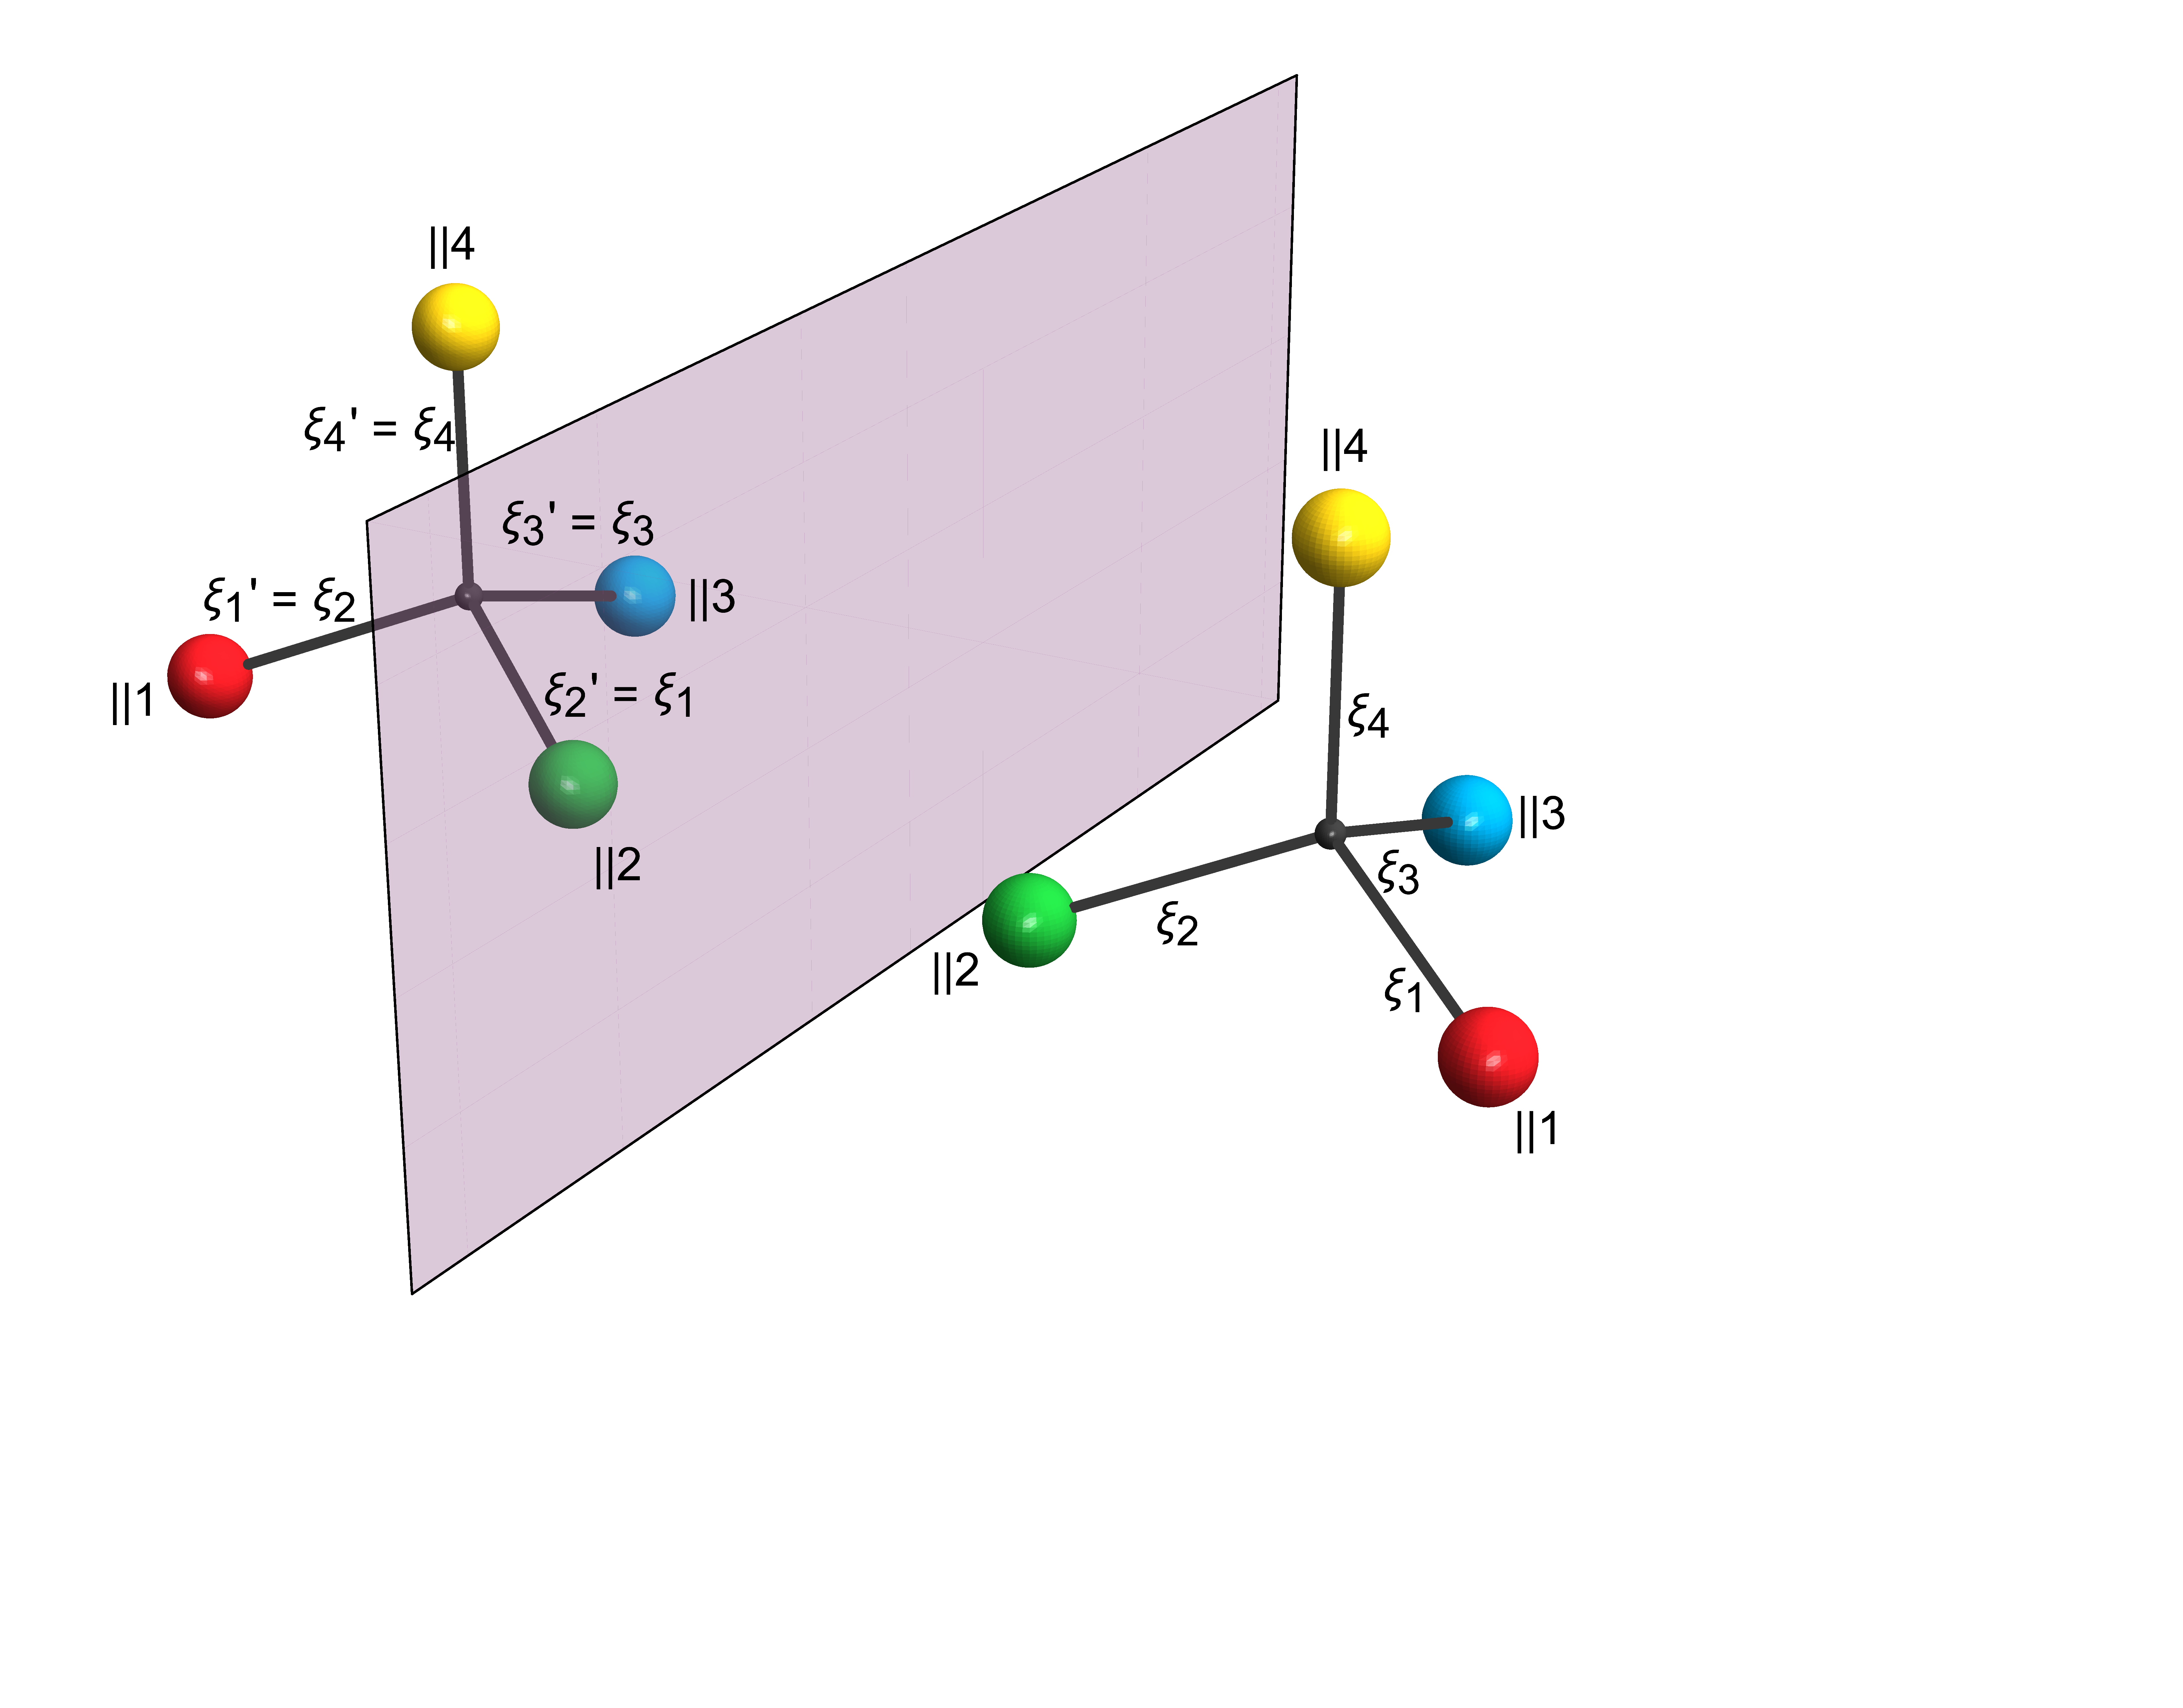
\includegraphics[scale = 0.4]{/Users/philipp/Documents/GitHub/stage_cmap/images/reflection.png}
\caption{La refléxion $S_{12}$ appliquée à \textsc{SPr4} dans l'orientation de référence correspondant à l'échangement $(||1 \leftrightsquigarrow ||2)$ }
\label{fig:reflection of swimmer}
\end{figure}
\end{frame}

\begin{frame}{Symétries - Permutation des bras}
\begin{itemize}
\item On trouve par un calcul technique
\begin{align}
	 F_c(P_{ij} \xi) = S_{ij} F_c(\xi) P_{ij} \text{ et } F_{\theta}(P_{ij} \xi) = - S_{ij} F_{\theta}(\xi) P_{ij}. \forall \xi \in \M.
\end{align}

\item Attention: Il faut toujours choisir la base canonique $\mathcal{E} = (e_1, e_2,e_3, e_4)$ pour $\R^4$ et la base $\mathcal{L} = (L_1, L_2, L_3)$ avec

\renewcommand{\arraystretch}{0.7}
\begin{align}
	&L_1 =  \left(\begin{array}{ccc}
	0 & 0 & 0 \\ 
	0 & 0 & -1 \\ 
	0 & 1 & 0
	\end{array}  \right ),
	&L_2 =  \left (\begin{array}{ccc}
	0 & 0 & 1 \\ 
	0 & 0 & 0 \\ 
	-1 & 0 & 0
	\end{array}  \right ),\\
	&L_3 = \left (\begin{array}{ccc}
	0 & -1 & 0 \\ 
	1 & 0 & 0 \\ 
	0 & 0 & 0
	\end{array}  \right ),
\end{align}
\renewcommand{\arraystretch}{1}
pour justifier la notation!
\end{itemize}
\end{frame}


\section[Petites courbes]{Régime des petites courbes de contrôle}

\begin{frame}{Petites courbes - Développement limité}
\begin{itemize}
\item On a la factorisation
\begin{equation}
\label{eq: reminder control system}
	F_{c}(R, \zeta) = R F_{c}(\zeta) \text{ et } F_{\theta}(R, \xi) = R F_{\theta}(\zeta), \forall R \in \SO(3),
\end{equation}
où $F_{c}(\zeta) := F_c(I, \zeta)$ et $F_{\theta}(\zeta) := F_{\theta}(I, \zeta)$.
\item On suppose que $\zeta = \xi_0 + \xi$, $\xi_0$ avec toutes les composantes égales
\item $F_{c, \xi_0}(\xi) := F_{c}(\xi_0 + \xi)$, $F_{\theta, \xi_0}(\xi) := F_{\theta}(\xi_0 + \xi)$
\item Résultat de \cite{Alouges2013}: $F$ et donc aussi $F_{c, \xi_0}, F_{\theta, \xi_0}$ analytiques
\item On fait le développement limité
\begin{align}
\label{eq: spatial control expansion}
	F_{c, \xi_0}(\xi)\eta &= F_{c, 0} \eta  + \h_{c,0}(\xi \otimes \eta) + \mathcal{O}(|\xi|)\eta\\
\label{eq: angular control expansion}
	F_{\theta, \xi_0}(\xi) \eta &= F_{\theta, 0} \eta + \h_{\theta, 0}(\xi \otimes \eta) + \mathcal{O}(|\xi|)\eta,
\end{align}
pour tout $\eta \in \R^4$.
\end{itemize}
\end{frame}

\begin{frame}{Petites courbes - Développement limité}
\begin{itemize}
\item Substitution des conditions de symétrie de $F$ dans le développement limité fournit
\begin{align}
\label{eq:zeroth_order_sym}
	F_{c,0} &= S_{ij} F_{c,0} P_{ij}\\
	F_{\theta, 0} &= -S_{ij} F_{\theta, 0} P_{ij}
\end{align}
\begin{align}
\label{eq:first_order_sym}
\h_{c,0}(P_{ij} \xi\otimes \eta) &= S_{ij} \h_{c,0}(\xi \otimes P_{ij} \eta), &\forall \xi, \eta \in \R^4\\
\h_{\theta,0}(P_{ij} \xi \otimes \eta) &= -S_{ij} \h_{\theta,0}(\xi \otimes P_{ij} \eta), &\forall \xi, \eta \in \R^4
\end{align}
\item On veut déterminer les espaces de solutions de ces systèmes d'équations vectorielles.
\end{itemize}
\end{frame}

\begin{frame}{Petites courbes - Termes d'ordre zéro}
\begin{itemize}
\item Calcul élémentaire pour trouver 
\begin{equation}
	F_{c,0} = \mathfrak{a} (z_1 |z_2| z_3|z_4),
\end{equation}
avec $\mathfrak{a} \in \R$ ou bien
\begin{equation}
	F_{c,0} = - 3 \sqrt{3} \mathfrak{a} [\tau_1| \tau_2 |\tau_3]^T,
\end{equation}
où $\tau_1 : = \tfrac{1}{\sqrt{6}}(-2,1,1,0)^T$, $\tau_2 := \tfrac{1}{\sqrt{2}}(0,1,-1,0)^T$, $\tau_{3}:= \tfrac{1}{2 \sqrt{3}} (1,1,1,-3)^T$ forment une base orthonormale ensemble avec $\tau_4:= \tfrac{1}{2}(1,1,1,1)^T$. Cette base sera utile plus tard.
\item Des arguments similaires montrent que $F_{\theta, 0} = 0$, ce qui est intuitivement clair.
\end{itemize}
\end{frame}

\begin{frame}{Petites courbes - Termes d'ordre un}
\begin{itemize}
\item Même approche que \cite{Alouges2017}
\begin{align}
A_k &:= (\h_{c,0}(e_i \otimes e_j)\cdot \hat{e}_k)_{i,j \in \N_4}, k \in \N_3\\
B_k &:= (\h_{\theta,0}(e_i \otimes e_j)\cdot L_k)_{i,j \in \N_4}, k \in \N_3.
\end{align}

\item Ainsi, on a pour tout $\xi, \eta \in \R^4$
\begin{align}
\label{eq: matrix representation of spatial first order term}
	\h_{c,0}(\xi \otimes \eta) = \sum_{k \in \N_3}(A_k \eta \cdot \xi)\hat{e}_k, \\
\label{eq: matrix representation of angular first order term}
	\h_{\theta, 0}(\xi \otimes \eta) = \sum_{k \in \N_3}(B_k \eta \cdot \xi) L_k.
\end{align}

\item À lieu de calculer directement les matrices $A_k$ et $B_k$, on a calculé leurs parties symétriques et anti-symétriques en utilisant des arguments de symétrie. Notons les parties anti-symmétriques
\begin{align}
M_k &:= \frac{1}{2}[A_k - A_k^T], k \in \N_3\\
M_{k + 3} &:= \frac{1}{2}[B_k - B_k^T], k \in \N_3.
\end{align}

\end{itemize}
\end{frame}

\begin{frame}{Petites courbes - Termes d'ordre un}
Dans la suite seulement les parties anti-symétrique seront importantes:
\renewcommand{\arraystretch}{0.7}
\begin{align}
\label{eq: M1 and M2}
&M_1 = \alpha \left ( \begin{array}{cccc}
0 & 3 & 3 & 2 \\ 
-3 & 0 & 0 & -1 \\ 
-3 & 0 & 0 & -1 \\ 
-2 & 1 & 1 & 0
\end{array} \right ) ,\\
&M_2 = \sqrt{3} \alpha \left (
\begin{array}{cccc}
0 & 1 & -1 & 0 \\ 
-1 & 0 & -2 & -1 \\ 
1 & 2 & 0 & 1 \\ 
0 & 1 & -1 & 0
\end{array} \right),\\
&M_3 = 2 \sqrt{2} \alpha \left (
\begin{array}{cccc}
0 & 0 & 0 & -1 \\ 
0 & 0 & 0 & -1 \\ 
0 & 0 & 0 & -1 \\ 
1 & 1 & 1 & 0
\end{array} 
\right ).
\end{align}
\renewcommand{\arraystretch}{1}
\end{frame}

\begin{frame}{Petites courbes - Termes d'ordre un}
\renewcommand{\arraystretch}{0.7}
\begin{align}
\label{eq: M4 and M5}
	&M_4 = \delta \left (
	\begin{array}{cccc}
	0 & 1 & 1 & 0 \\ 
	-1 & 0 & -2 & 3 \\ 
	1 & 2 & 0 & -3 \\ 
	0 & -3 & 3 & 0
	\end{array} 
	\right ),\\
	&M_5 = \sqrt{3} \delta \left ( \begin{array}{cccc}
	0 & -1 & -1 & 2 \\ 
	1 & 0 & 0 & -1 \\ 
	1 & 0 & 0 & -1 \\ 
	-2 & 1 & 1 & 0
	\end{array} \right ) ,\\
&M_6 = 2 \sqrt{2} \delta \left (\begin{array}{cccc}
0 & 1 & -1 & 0 \\ 
-1 & 0 & 1 & 0 \\ 
1 & -1 & 0 & 0 \\ 
0 & 0 & 0 & 0
\end{array}  \right )
\end{align}
\renewcommand{\arraystretch}{1}
\end{frame}

\begin{frame}{Petites courbes - Linéarisation}
\begin{itemize}
\item Restriction de l'espace des contrôles à $H^1_{\sharp}(J, \R^4)$, où $J := [0, 2\pi]$
\item $\langle f \rangle := (2 \pi)^{-1 }\int_{J} f(t) d t$ pour $f \in H^1_{\sharp}(J, \R^4)$

\item Dans la partie précédente, on a trouve que pour $\zeta = \xi_0 + \xi$, on a autour de $\xi = 0$
 \begin{align}
 \label{eq: dynamics first approx}
 \begin{cases}
 	\dot{c} &= R F_{c,0} \dot{\xi} + R \sum_{k \in \N_3}(A_k \dot{\xi} \cdot \xi)\hat{e_k}\\
 	\dot{R} &= R \sum_{k \in \N_3} (B_k \dot{\xi} \cdot \xi) L_k.
 \end{cases}
 \end{align}
\end{itemize}

\end{frame}

\begin{frame}{Petites courbes - Linéarisation}
\begin{itemize}
\item On définit les déplacements nets par
\begin{align}
	\delta c: &H_{\sharp}^1(J,\R^4) \to \R^3, &
	\delta R: & H_{\sharp}^1(J,\R^4) \to \so(3)\\
	&\xi \mapsto 2\pi \langle \dot{c} (\xi) \rangle \nonumber, &
	&\xi \mapsto 2 \pi \langle \dot{R}(\xi) \rangle \nonumber
\end{align}
\item Impossible d'évaluer ces expressions exactement à cause du $R$ dans (\ref{eq: dynamics first approx})!

\item Un argument du \emph{calcul chronologique} permet de linéariser autour de $R_0 = I$. Ainsi, on trouve

\begin{proposition}
\label{prop:net displacement}
Pour tout $\xi \in H_\sharp^1(J, \R^4)$, dans un voisinage de $0 \in H_{\sharp}^{1}(J, \R^4)$, on a les estimes suivants
\begin{equation}
\begin{aligned}
\delta c(\xi) &= 2 \pi \sum_{k \in \N_3} \langle A_k \dot{\xi} \cdot \xi \rangle \hat{e}_k + \mathcal{O}(||\xi||_{H^1_{\sharp}}^3),\\
\delta R(\xi) &= 2 \pi \sum_{k \in \N_3} \langle B_k \dot{\xi} \cdot \xi \rangle L_k + \mathcal{O}(||\xi||^4_{H_\sharp^1}).
\end{aligned}
\end{equation}
\end{proposition}
\end{itemize}

\end{frame}

\begin{frame}{Petites courbes - Linéarisation}
\begin{itemize}
\item $A$ symétrique $\overset{I.P.P.}{\implies} \langle A \xi \cdot \dot{\xi} \rangle = - \langle A \xi \cdot \dot{\xi} \rangle = 0$ et donc
\begin{align}
\langle A_k \dot{\xi} \cdot \xi \rangle &= \langle M_k \dot{\xi} \cdot \xi \rangle, &\forall k \in \N_3\\
\langle B_k \dot{\xi} \cdot \xi \rangle &= \langle M_{k + 3} \dot{\xi} \cdot \xi \rangle, &\forall k \in \N_3
\end{align}

\item Si on note $\{f_k\}_{k \in \N_6}$ la base canonique de $\R^6$, un calcul montre que
\begin{align}
\label{eq: net displacement}
\frac{\delta p}{2 \pi}= - 2  \sqrt{6} \alpha \sum_{k \in \N_3}\langle \det( \xi | \dot{\xi} | \tau_{k+1} | \tau_{k+2})\rangle f_k \nonumber \\ - 2  \sqrt{6} \delta \sum_{k \in \N_3}\langle \det ( \xi | \dot{\xi} | \tau_{k} | \tau_{4})\rangle f_{k + 3},
\end{align}
où $k$ pris mod 3.

\item En particulier, on peut décrire les déplacements nets à deux paramètres scalaires près.

%\item Par un calcul on obtient
%\begin{align}
%  M_k \dot{\xi} \cdot \xi &= - 2 \sqrt{6} \,\alpha \det( \xi | \dot{\xi} | \tau_{k+1} | \tau_{k+2}),  & & k \in \N_3\\
%  M_{3 + k} \dot{\xi} \cdot \xi &= - 2 \sqrt{6} \,\delta \det ( \xi | \dot{\xi} | \tau_{k} | \tau_{4}), & & k \in \N_3,
%\end{align}
%où $\{\tau_l\}_{l \in \N_4}$ est la base orthonormée vue précédemment et $k$ est pris mod 3.
\end{itemize}
\end{frame}


\section{Optimisation}

\begin{frame}{Optimisation - Notation}
\begin{itemize}
\item Définition d'efficacité selon Lighthill \cite{Lighthill1952}: \emph{Les mouvements optimaux sont ceux qui minimisent la dissipation d'énergie cinétique en atteignant un déplacement net prescrit.}

\item La dissipation d'énergie due à un mouvement $\xi \in H^1_{\sharp}(J, \R^4)$ s'écrit par une fonctionnelle d'énergie appropriée
\begin{equation}
 \mathcal{G}(\xi) := \int_{J} \mathfrak{g}(\xi(t))\dot{\xi}(t) \cdot \dot{\xi}(t) \dd t.
\end{equation}

\item Sous l'hypothèse des petites courbes de contrôle, on peut supposer que $\mathfrak{g}(\xi) = \mathfrak{g}(0) + o(1)$, avec $\mathfrak{g}(0)$ une matrice symétrique définie positive dans $M_{4 \times 4}(\R)$. Ainsi, l'énergie s'écrit
\begin{equation}
\label{eq: linearized energy functional}
	\mathcal{G}(\xi) := \int_{J} Q_{\mathfrak{g}}(\dot{\xi}(t))\dd t,
\end{equation}
avec $Q_{\mathfrak{g}}(\eta) := \mathfrak{g}(0)\eta \cdot \eta$.
\end{itemize}
\end{frame}

\begin{frame}{Optimisation - Notation}
\begin{itemize}
\item Les propriétés de symétrie des équations Stokes impliquent en particulier que
\begin{align}
	Q_{\mathfrak{g}}(P_{ij} \eta) = Q_{\mathfrak{g}}(\eta),\; i,j \in \N_4.
\end{align}

\item La matrice $G$ représentant $Q_{\mathfrak{g}}$ est de la forme suivante:
\begin{equation}
G = \left ( \begin{array}{cccc}
\kappa & h & h & h \\ 
h & \kappa & h & h \\ 
h & h & \kappa & h \\ 
h & h & h & \kappa
\end{array} \right ),
\end{equation}
pour deux paramètres $h$ et $\kappa > \max(h, -3h)$.
\item On a $G \tau_k = (\kappa - h ) \tau_k$ pour $k \in  \N_3$ et $G \tau_4 = (\kappa + 3h) \tau_4$
\item On notera $\mathfrak{g}_1 := \mathfrak{g}_2 := \mathfrak{g}_3 := \kappa - h$ et $\mathfrak{g}_4 := \kappa + 3h$ t.q.
\begin{eqnarray}
G = U \Lambda_{\mathfrak{g}} U^T, & U := [\tau_1 | \tau_2 |\tau_3 |\tau_4], & \Lambda_{\mathfrak{g}} := \diag(\mathfrak{g}_i).
\end{eqnarray}
\end{itemize}
\end{frame}


\begin{frame}{Optimisation - Notation}
On face le problème d'optimisation:
Minimiser $ \int_{J} Q_{\mathfrak{g}}(\dot{\xi}(t)) \dd t$ sous la contrainte
\begin{align}
\label{eq: constraint}
\delta p = \mathfrak{h}_{c} \sum_{k \in \N_3}\left ( \int_{J} \det( \xi(t) | \dot{\xi}(t) | \tau_{k+1} | \tau_{k+2}) \dd t \right ) f_k\\
	+ \mathfrak{h}_{\theta}  \sum_{k \in \N_3}\left ( \int_{J} \det ( \xi(t) | \dot{\xi}(t) | \tau_{k} | \tau_{4}) \dd t\right ) f_{k + 3} \nonumber
\end{align}
avec $\mathfrak{h}_c = - 2 \sqrt{6} \alpha$ et $\mathfrak{h}_{\theta} = - 2 \sqrt{6} \delta$.
\end{frame}


\begin{frame}{Optimisation - Bivecteurs de $\R^4$}
\begin{figure}[h]
\center
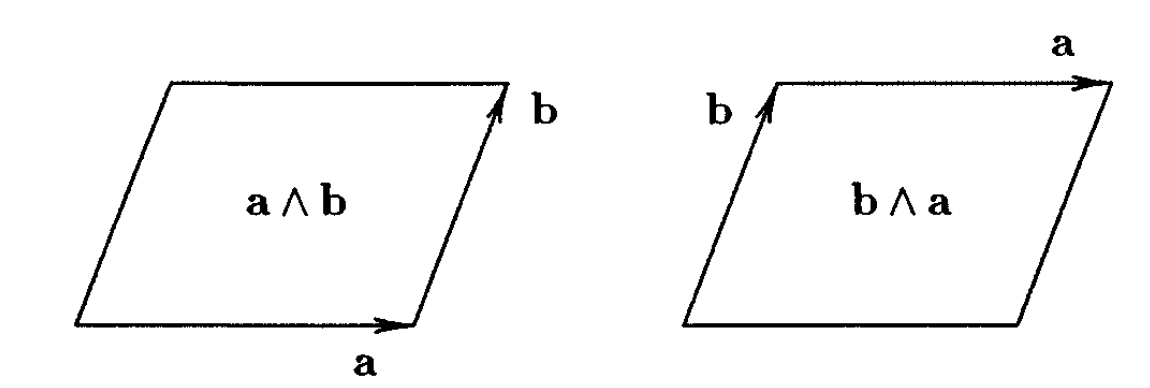
\includegraphics[scale=0.5]{/Users/philipp/Documents/GitHub/stage_cmap/tex/Présentation/images/bivecteurs.png}
\caption{Affichage d'un bivecteur dans $\R^3$ \cite{Lounesto2006}}
\end{figure}
\begin{itemize}
\item Les bivecteurs forment un espace vectoriel $\bigwedge^2 \R^3$ avec une base donnée par
\begin{equation}
 \{\hat{e}_1 \wedge \hat{e}_2, \hat{e}_1 \wedge \hat{e}_3, \hat{e}_2 \wedge \hat{e}_3\},
\end{equation}
si $\{\hat{e}_1, \hat{e}_2, \hat{e}_3\}$ est une base de $\R^3$.
\end{itemize}
\end{frame}


\begin{frame}{Optimisation - Bivecteurs de $\R^4$}
\begin{itemize}
\item Le produit scalaire est donné par
\begin{equation}
( u_1 \wedge u_2 , v_1 \wedge v_2 ) = \det \left (\begin{array}{cc}
u_1 \cdot v_1 & u_1 \cdot v_2 \\ 
u_2 \cdot v_1 & u_2 \cdot v_2
\end{array}  \right).
\end{equation}

\item La norme d'un bivecteur $\omega = \omega_{12} \hat{e}_1 \wedge \hat{e}_2 + \omega_{13} \hat{e}_1 \wedge \hat{e}_3 + \omega_{23} \hat{e}_2 \wedge \hat{e}_3$ est donnée par
\begin{equation}
|\omega| = \sqrt{\omega_{12}^2 + \omega_{13}^2 + \omega_{23}^2}.
\end{equation}

\item Ces idées se généralisent facilement à dimension supérieure. En effet, si $\{e_1, e_2, e_3, e_4\}$ est la base canonique de $\R^4$, alors une base de l'espace $\bigwedge^2 \R^4$ est donnée par
\begin{equation}
\{e_{12}, e_{13}, e_{14}, e_{23}, e_{24}, e_{34}\},
\end{equation}
où  $e_{ij} := e_i \wedge e_j$.
\end{itemize}
\end{frame}

\begin{frame}{Optimisation - Bivecteurs de $\R^4$}
\begin{itemize}
\item Différence fondamentale: $\bigwedge^2 \R^3 \simeq \R^3$, mais $\bigwedge^2 \R^4 \not \simeq \R^4$

\item $\bigwedge^2  \R^3 \simeq \R^3$ implique que tout $\omega \in \bigwedge^2 \R^3$ est \emph{simple}, c'est-à-dire que
\begin{equation}
\forall \omega \in \bigwedge^2 \R^3 \exists u,v \in \R^3: \omega = u \wedge v.
\end{equation}

\item Ceci n'est plus le cas pour $\bigwedge^2\R^4$, e.g. $e_{12} + e_{34} \in \bigwedge^2\R^4$ n'est pas simple

%\item Tout bivecteur de $\R^4$ est la somme d'au plus deux bivecteurs simples et orthogonaux

\item Après passage en Fourier, la contrainte s'identifiera à un bivecteur de $\R^4$. Si celui-ci est simple, nous pourrons résoudre le problème d'optimisaton de façon similaire à \cite{Alouges2017}.

%\item Critère pour trouver des bivecteurs simples:
%\begin{lemma}
%\label{lem:simple bivector}
%un bivecteur $\omega \in \bigwedge^2 \R^4$ est simple si et seulement si $\omega \wedge \omega = 0$.
%\end{lemma}
\end{itemize}
\end{frame}

\begin{frame}{Optimisation - G-Orthogonalisation}
\begin{itemize}
\item On pose $\eta(t) := U^T \xi(t) \in H^1_{\sharp}(J, R^4)$, ce qui permet d'écrire
\begin{equation}
\label{eq: G-orth energy functional}
\mathcal{G}_{U}(\eta) = \int_{J} \Lambda_{\mathfrak{g}} \dot{\eta}(t) \cdot \dot{\eta}(t) \dd t,
\end{equation}
avec $\mathcal{G}_{U}(\eta) := \mathcal{G}(\xi) = \mathcal{G}(U \eta)$.

%\item Pour la contrainte, on observe que
%\begin{eqnarray}
%\det(\xi |\dot{\xi} | \tau_i | \tau_j) =  \det U \det (\eta | \dot{\eta} | e_i | e_j) = \det(\dot{\eta} | \eta | e_i |e_j),& \det U = -1.
%\end{eqnarray}

%\item Puis, un calcul montre que
%\begin{align}
%\det(\dot{\eta} | \eta | e_k |e_4) &= (\dot{\eta} \wedge \eta, e_{k + 1} \wedge e_{k+2}), & k \in \N_3\\
%\det(\dot{\eta} |\eta | e_{k + 1} |e_{k + 2}) &= (\dot{\eta} \wedge \eta, e_k \wedge e_4), & k \in \N_3
%\end{align}
%\item Si on envoie maintenant la base canonique $\{f_k\}_{k \in \N_6}$ sur la base ordonnée $(e_{14}, e_{24}, e_{34}, e_{23}, e_{31}, e_{12})$ 
%de $\bigwedge^2 \R^4$, la contrainte s'écrit

\item Si on envoie $\{f_k\}_{k \in \N_6}$ vers une certaine base de $\bigwedge^2 \R^4$, on trouve
\begin{equation}
\label{eq: G-orth constraint}
\Lambda_{\mathfrak{h}}^{-1} \delta p = \int_{J} \dot{\eta}(t) \wedge\eta(t) \dd t,
\end{equation}
avec $\Lambda_{\mathfrak{h}} := \diag(\mathfrak{h}_{c}, \mathfrak{h}_{c}, \mathfrak{h}_{c}, \mathfrak{h}_{\theta}, \mathfrak{h}_{\theta}, \mathfrak{h}_{\theta})$.

\item Ainsi, le problème d'optimisation devient: Minimiser $ \int_{J}\Lambda_{\mathfrak{g}} \dot{\eta}(t) \cdot \eta(t) \dd t $ sous la contrainte 
\begin{equation}
\Lambda_{\mathfrak{h}}^{-1} \delta p = \int_{J} \dot{\eta}(t) \wedge\eta(t) \dd t.
\end{equation}
\end{itemize}
\end{frame}


\begin{frame}{Optimisation - Passage en Fourier}
\begin{itemize}
\item On passe en Fourier car les courbes de contrôle sont $2 \pi$- périodiques par définition. On notera
\begin{equation}
\dot{\ell}^2(\R^4) := \{\mathbf{u} = (u_n)_{n \in \N} \mid (n u_n)_{n \in \N} \in \ell^2(\R^4)\}.
\end{equation}

\item Expansion en série de Fourier:
\begin{equation}
\eta(t) := \frac{1}{2} a_0 + \sum_{n \in \N} \cos(nt) a_n + \sin(n t) b_n,
\end{equation}
avec $(a_n, b_n)_{n \in \N} \in \dot{\ell}^2(\R^4) \times \dot{\ell}^2(\R^4)$.
\end{itemize}
\end{frame}

\begin{frame}{Optimisation - Passage en Fourier}
\begin{itemize}
\item Substitution dans la fonctionnelle d'énergie et la contrainte fournit
\begin{align}
\mathcal{G}_{U} (\eta) := \int_{J} \Lambda_{\mathfrak{g}} \dot{\eta}(t) \cdot \dot{\eta} dt &= \pi \sum_{n  \in \N} n^2(\Lambda_{\mathfrak{g}} a_n \cdot a_n + \Lambda_{\mathfrak{g}} b_n \cdot b_n)  \\  &=
\frac{1}{2} ||\mathbf{u}||_{\ell^2(\R^4)}^2 + \frac{1}{2} ||\mathbf{v}||_{\ell^2(\R^4)}^2,
\end{align}
où on a posé
\begin{align}
\label{eq:relation Fourier coeffs of eta}
	\mathbf{u} &:= (u_n)_{n \in \N} := \sqrt{2 \pi \Lambda_{\mathfrak{g}}}(n a_n)_{n \in \N},\\
	\mathbf{v} &:= (v_n)_{n \in \N} := \sqrt{2 \pi \Lambda_{\mathfrak{g}}} (n b_n)_{n \in \N},
\end{align}
et
\begin{equation}
\sqrt{\det \Lambda_{\mathfrak{g}}} (\Lambda_{\mathfrak{h}} \tilde{\Lambda}_{\mathfrak{g}})^{-1} \delta p = \sum_{n \in \N} \frac{v_n  \wedge u_n}{n},
\end{equation}
avec $\tilde{\Lambda}_{\mathfrak{g}} := \diag(\mathfrak{g}_c, \mathfrak{g}_c, \mathfrak{g}_c, \sqrt{\mathfrak{g}_c \mathfrak{g}_{\theta}}, \sqrt{\mathfrak{g}_c \mathfrak{g}_{\theta}}, \sqrt{\mathfrak{g}_c  \mathfrak{g}_{\theta}})$, où $\mathfrak{g}_1 :=\mathfrak{g}_2 := \mathfrak{g}_3 := \mathfrak{g}_c$ et $\mathfrak{g}_4 := \mathfrak{g}_\theta$.
\end{itemize}
\end{frame}

\begin{frame}{Optimisation - Passage en Fourier}
\begin{itemize}
\item Ceci prouve le résultat suivant:
\begin{proposition}
\label{prop: l2-minimization}
La $H_{\sharp}^1(J, \R^4)$-minimisation de la fonctionelle $\mathcal{G}_U$ donnée par (\ref{eq: G-orth energy functional}) sous la contrainte (\ref{eq: G-orth constraint}) équivaut la minimisation de la fonctionnelle
\begin{equation}
\label{eq:l2-energy}
	\mathcal{F}(\mathbf{u}, \mathbf{v}) := \frac{1}{2} ||\mathbf{u} ||^2_{\ell^2(\R^4)} + \frac{1}{2} ||\mathbf{v}||^2_{\ell^2(\R^4)},
\end{equation}
définie sur l'espace produit $\ell^2(\R^4) \times \ell^2(\R^4)$ et sous la contrainte
\begin{equation}
\label{eq:l2-constraint}
\sum_{n \in \N} \frac{1}{n} v_n \wedge u_n = \omega \text{ with } \omega := \sqrt{\det \Lambda_{\mathfrak{g}}}(\Lambda_{\mathfrak{h}} \tilde{\Lambda}_{\mathfrak{g}})^{-1} \delta p,
\end{equation}
où $\delta p \in \R^3 \times \so(3)$ est un déplacement net préscrit en position.
\end{proposition}

\item On observe que  $\omega \in \bigwedge^2\R^4$ et que $\omega$ est simple si et seulement si $\delta p$ est simple.
\end{itemize}
\end{frame}

\begin{frame}{Optimisation - Passage en Fourier}
\begin{itemize}
\item On veut réduire ce problème à un problème en dimension finie (c.f. \cite{Alouges2017}), i.e. trouver pour toute paire de suites de coefficients de Fourier $(\mathbf{u}, \mathbf{v}) \in \ell^2(\R^4) \times \ell^2(\R^4)$ un nombre fini de coefficients de Fourier, i.e. $(\tilde{\mathbf{u}}, \tilde{\mathbf{v}}) \in c_{00}(\R^4) \times c_{00}(\R^4)$ tel  que
\begin{align}
	\mathcal{F}(\tilde{\mathbf{u}}, \tilde{\mathbf{v}}) = \mathcal{F}(\mathbf{u}, \mathbf{v}) \text{ et }  \sum_{n = 1}^{N} \frac{1}{n} \tilde{v}_n \wedge \tilde{u}_n = \sum_{n \in \N} \frac{1}{n} v_n \wedge u_n.
\end{align}
\item $\to$ Problème d'optimisation dans $\R^N$
\end{itemize}
\end{frame}

\section{Le cas simple}

\begin{frame}{Le cas simple - Réduction à dimension finie}
Supposons que $\omega = x\wedge y$ est un bivecteur simple. En effet, de manière similaire à \cite{Alouges2017}, on trouve le résultat suivant:

\begin{proposition}
\label{prop:simple reduction}
Si $\omega$ est un bivecteur simple, alors pour tout $(\mathbf{u}, \mathbf{v}) \in \ell^2(\R^4) \times \ell^2(\R^4)$ tel que la contrainte (\ref{eq:l2-constraint}) soit satisfaite, il existe deux vecteurs $u,v \in \R^4$ tels que pour les suites $\mathbf{u}_{\star} := \mathbf{e}_1 u$ et $\mathbf{v}_\star := \mathbf{e}_1 v \in \ell^2(\R^4)$ on ait 
\begin{equation}
\mathcal{F}(\mathbf{u_{\star}}, \mathbf{v_{\star}}) = \mathcal{F}(\mathbf{u}, \mathbf{v}) \text{ and } v \wedge u = \omega.
\end{equation}
\end{proposition}
\end{frame}

\begin{frame}{Le cas simple - Théorème final}
Ensuite, la résolution du problème d'optimisation en dimension finie fournit le résultat final:
\begin{theorem}
\label{thm:optimal control curves in the simple case}
Soit $\delta p \in \R^3 \times \so(3) \simeq \bigwedge^2 \R^4$ un déplacement net prescrit. De plus, supposons que $\delta p = x \wedge y$ soit un bivecteur simple. Alors, tout minimiseur $\xi \in H_{\sharp}^1(J, \R^4)$ de la fonctionnelle d'énergie (\ref{eq: linearized energy functional}) sous la contrainte (\ref{eq: constraint}) est de la forme
\begin{equation}
\xi(t) := (\cos t) a + (\sin t) b,
\end{equation}
i.e. une ellipse de $\R^4$ centrée à l'origine et contenu dans le plan défini par les vecteurs $a$ et $b$. On obtient les vecteurs $a,b \in \R^4$ comme ce qui suit:

\end{theorem}
\end{frame}

\begin{frame}{Le cas simple - Théorème final}
\begin{enumerate}
\item On calcule le vecteur $\omega$ via la relation
\begin{equation}
\omega := \diag \left (\frac{\sqrt{\mathfrak{g}_c \mathfrak{g}_{\theta}}}{\mathfrak{h}_c}, \frac{\sqrt{\mathfrak{g}_c \mathfrak{g}_{\theta}}}{\mathfrak{h}_c}, \frac{\sqrt{\mathfrak{g}_c \mathfrak{g}_{\theta}}}{\mathfrak{h}_c}, \frac{\mathfrak{g}_c}{\mathfrak{g}_\theta}, \frac{\mathfrak{g}_c}{\mathfrak{g}_\theta}, \frac{\mathfrak{g}_c}{\mathfrak{g}_\theta} \right ) \delta p = \tilde{x} \wedge \tilde{y}.
\end{equation}
Puis on considère deux vecteurs $u,v \in \Span\{\tilde{x}, \tilde{y}\}$ tels que
\begin{equation}
\label{eq:global minimizer condition}
|u|^2 = |v|^2 = |\omega| \text{ and } u \cdot v = 0.
\end{equation}

\item On pose $\hat{\omega} := \omega/|\omega|$ et on calcule les vecteurs a$a$ et $b$ via les relations
\begin{equation}
\label{eq:global minimizer form}
\begin{aligned}
a := \frac{U \Lambda_{\mathfrak{g}}^{-1/2}}{\sqrt{2 \pi}} u,&& b := \frac{U \Lambda_{\mathfrak{g}}^{-1/2}}{\sqrt{2 \pi}} v.
\end{aligned}
\end{equation}
\end{enumerate}
Alors, on a $ v \wedge u = \omega$ et the la valeur minimum de $\mathcal{G}$ est égale à $|\omega|$.

En outre, les vecteurs $a$ et $b$ sont $\mathfrak{g}$-orthogonaux, i.e. par rapport au produit scalaire défini pour tout $x,y \in \R^4$ par $(x, y)_{\mathfrak{g}} := 2 \pi \Lambda_{\mathfrak{g}} x \cdot y$, et ils on la même $\mathfrak{g}$-norme $|a|_{\mathfrak{g}}^2 = |b|_{\mathfrak{g}}^2 = |\omega|$. 
\end{frame}

%\begin{frame}{Le cas simple - Exemples de cas simples}
%\begin{itemize}
%\item Naturellement, on se pose la question dans quelles situations $\omega$ est simple
%
%\item On remarque que ce critère est un particulier toujours satisfait dès que les composantes de $\omega$ correspondant à un certain indice valent zéro, e.g. $\omega_{i4} = 0$ pour $i \in \N_3$
%
%\item Ceci fournit quatre sous-espaces $D^*_{ijk}$ de $\bigwedge^2 \R^4$ consistant uniquement de bivecteurs simples. Par inspection de notre base choisie pour $\bigwedge^2 \R^4$, on trouve les correspondances suivantes:
%\begin{align*}
%D^{*}_{123} &\longleftrightarrow\text{ rotations autour toutes les trois axes } \hat{e}_1, \hat{e}_2, \hat{e}_3\\
%D^{*}_{124} &\longleftrightarrow \text{ translation dans le plan de $\hat{e}_1$ et $\hat{e}_2$, rotation autour de $\hat{e}_3$}\\
%D^{*}_{134} &\longleftrightarrow  \text{ translation dans le plan de $\hat{e}_1$ et $\hat{e}_3$, rotation autour de $\hat{e}_2$ }\\
%D^{*}_{234} &\longleftrightarrow  \text{ translation dans le plan de $\hat{e}_2$ et $\hat{e}_3$, rotation autour de $\hat{e}_1$ }
%\end{align*}
%
%\item En revanche, le bivecteur non-simple $e_{12} + e_{34}$ correspond au déplacement net $e_3 + L_3$, c'est-à-dire un mouvement de vis. Pour ce genre de mouvements on a besoin d'une solution pour le cas général.
%\end{itemize}
%\end{frame}

\section{Conclusions et perspectives}

\begin{frame}{Conclusions}
\begin{itemize}
\item Détermination des symétries du système dynamique qui décrit le micro-nageur \textsc{SPr4} à l'aide des propriétés des équations de Stokes.

\item Identification de la dynamique de \textsc{SPr4} à termes d'ordre élevé près sous l'hypothèse des petites courbes de contrôle ainsi que le déplacement net. Il reste cinq paramètres scalaires inconnus.

\item Structure des courbes de contrôle optimales dans un cas particulier qui décrit déjà une variétés de déplacements nets.
\end{itemize}

\end{frame}


\begin{frame}{Conjecture}
\begin{itemize}
\item Pas de solution pour le problème d'optimisation général.

\item Conjecture: En général, les courbes de contrôle optimales sont des ellipses situées dans un ou au plus deux plans totalement orthogonaux de $\R^4$. En outre, la fréquence de la rotation dans un des deux plans et le double de la fréquence dans l'autre plan.
\end{itemize}
On a les raisons suivantes pour cette conjecture:
\begin{enumerate}
\item Dans le cas simple $\omega$ définit le plan dans lequel la courbe optimale est située. Or, un bivecteur non-simple représente deux plans totalement orthogonaux.
$\to$ Construire les quatre coefficients de Fourier à partir des deux plans définis par $\omega$
\end{enumerate}
\end{frame}

\begin{frame}
\begin{enumerate}
\setcounter{enumi}{1}
\item L'équation d'Euler-Lagrange associée au problème d'optimisation (c.f. \cite{DeSimone2011}) s'écrit:
\begin{equation}
G \ddot{\xi} - \Omega(\mu) \dot{\xi} = 0,
\end{equation}
avec $\Omega(\mu) = \sum_{k \in \N_6} \mu_k M_k$. La matrice $\Omega(\mu)$ étant toujours anti-symétrique, la solution est une rotation dans $R^4$, c'est-à-dire elle est située dans deux plans totalement orthogonaux.

\item La dernière partie de la conjecture suit d'un argument de regroupement des suites $\mathbf{u}$ et $\mathbf{v}$.
\end{enumerate}
\end{frame}

\begin{frame}{Perspectives}
\begin{itemize}
\item Prouver la conjecture ci-dessus

\item Faire l'approximation des bras longs comme dans \cite{Alouges2020} pour simplifier le système encore une fois et déterminer les paramètres inconnus en termes de $\xi_0$ et $a$
\end{itemize}
\end{frame}





\appendix

\section{Questions ?}

\begin{frame}[allowframebreaks]{References}

  \printbibliography

\end{frame}

\end{document}